
%                                                                 aa.dem
% AA vers. 6.1, LaTeX class for Astronomy & Astrophysics
% demonstration file
%                                                 (c) Springer-Verlag HD
%                                                revised by EDP Sciences
%-----------------------------------------------------------------------
%
\documentclass[]{aa} %
%\documentclass[referee]{aa} % for a referee version
%\documentclass[onecolumn]{aa} % for a paper on 1 column
%\documentclass[longauth]{aa} % for the long lists of affiliations
%\documentclass[rnote]{aa} % for the research notes
%\documentclass[letter]{aa} % for the letters
%
%\documentclass[structabstract]{aa}
%\documentclass[traditabstract]{aa} % for the abstract without structuration
                                   % (traditional abstract)
%
\usepackage{graphicx}
%%%%%%%%%%%%%%%%%%%%%%%%%%%%%%%%%%%%%%%%
\usepackage{txfonts}
%%%%%%%%%%%%%%%%%%%%%%%%%%%%%%%%%%%%%%%%
\usepackage{verbatim}
\usepackage{bm}
%\usepackage{natbib}
%\usepackage{amsmath}
%\usepackage{amsfonts}
%\usepackage{amssymb}
%\usepackage{MnSymbol}


\newcommand{\figref}[1]{Fig.~\ref{#1}}
\newcommand{\eqnref}[1]{Eq.~(\ref{#1})}


\begin{document}
%
   \title{The NIKA2 millimetre camera at the 30-meter IRAM telescope}
   \title{The NIKA2 millimetre camera: instrument description and first lights}

%   \subtitle{I. Overviewing the $\kappa$-mechanism}


\author
{
TBD
}


         \institute
	{
%$^1
Institut N\'eel, CNRS \& Universit\'{e} de Grenoble, BP 166, 38042 Grenoble, France
\and
%$^2
Institut de Plan\'etologie et dAstrophysique de Grenoble (IPAG), CNRS and Universit\'e de
Grenoble, BP 53, 38041 Grenoble, France
\and
%$^3 -->3
Laboratoire de Physique Subatomique et de Cosmologie,
Universit\'e de Grenoble,
  CNRS, Institut Polytechnique de Grenoble, 
  53, rue des Martyrs, Grenoble, France
\and
%$^4 -->4
Institut de RadioAstronomie Millim\'etrique, 300 rue de la Piscine, 38406 Saint Martin d'H\`eres, France
\and
%$^5 -->5
Cardiff School of Physics and Astronomy, Cardiff University, CF24 3AA, United Kingdom
\and
%$^6 -->6
Laboratoire AIM, CEA/IRFU, CNRS/INSU, UniversitÈ Paris Diderot, CEA-Saclay, 91191 Gif-Sur-Yvette, France 
\and
%$^7 -->7
Institut d'Astrophysique Spatiale (IAS), CNRS and Universit\'e Paris Sud, Orsay, France
\and
%$^8 -->8
Arizona State Uniuversity (ASU), Phoenix, USA
\and
%$^9  -->9
Institut de RadioAstronomie Millimetrique (IRAM), Granada, Spain
\and
%$^10
University College London, Department 
of Physics and Astronomy, Gower Street, London WC1E 6BT, UK
\and
%$^11
Universit\`a "La Sapienza", p.le A. Moro, Roma, Italy
             }

    \authorrunning{Monfardini et. al.}

   \date{Received December XX, XXXX; accepted XXX XX, XXXX}

% \abstract{}{}{}{}{}
% 5 {} token are mandatory

  \abstract
  % context heading (optional)
  % {} leave it empty if necessary
   {Millimetre-wave astronomy is today an indispensable tool for both general Astrophysics studies (e.g. star formation, galaxies morphology etc.) and Cosmology (e.g. CMB - Cosmic Microwave Background, high-redshift galaxies etc.). General purpose, large field-of-view instruments are needed to map the Sky at intermediate angular scales (e.g. angular resolution of the order of 10\,arc-sec) not accessibles by interferometers (e.g. ALMA in Chile, NOEMA on the French Alpes, ...) and space-borne surveys (Planck). In order to efficiently cover the bands ranging from 70 to 400\,GHz, accessible from the ground even for continuum observations, these instruments have to be installed at the focal plane of the largest single-dish telescopes that are placed at high altitude on selected dry observing sites. In this framework, we have constructed and deployed a multi-thousands pixels dual-band (150\,GHz and\,260 GHz) camera to image an instantaneous field-of-view of 6.5\,arc-min and map the linear polarisation at 260\,GHz.}
  % aims heading (mandatory)
   {First, providing a detailed description of this instrument, named NIKA2 (New IRAM KID Arrays 2), in particular focussing on the cryogenics, the optics  and the focal planes based on Kinetic Inductance Detectors (KID). The focal planes and part of the optics are cooled down to the nominal 150\,mK operating temperature by means of an ad-hoc dilution refrigerator. 
Secondly, presenting the performance measured on the Sky during the commissioning runs that took place between October 2015 and April 2017 at the 30-meters IRAM (Institut of Millimetric Radio Astronomy) telescope at Pico Veleta, near Granada.}
  % methods heading (mandatory)
   {We have targeted a number of astronomical sources. Starting from primary and secondary calibrators allowing extracting beam-maps and photometric adjustment, we have then gone to extended sources and faint objects. Both internal (electronics) and on-the-sky calibrations are applied. The general methods are described in the present paper and in others more focused on the NIKA2 sub-systems.}
  % results heading (mandatory)
   {NIKA2 has ben successfully deployed and commissioned, performing in-line with the ambitious expectations. In particular, we demonstrate the photometric and imaging performance and the mapping of faint extendes sources. Besides that, we demonstrated the ability of NIKA2 of detecting faint sources at the mJy level. A first successful science verification run has been achieved in April 2017, focussing on the mapping of galaxies clusters via the SZ effect. The instrument will be offered to the astronomical community during the coming winter and for the next 10\,years.
}
  % conclusions heading (optional), leave it empty if necessary
   {}


   \keywords{Superconducting detectors --
                mm-wave --
                kinetic-inductance --
                cosmic microwave background --
                large arrays
               }

   \maketitle
%
%________________________________________________________________

\section{Introduction}

In the last decades instrumental progress, and in particular the development of background limited detectors, has lead to a golden era of millimeter and sub-millimeter astronomy, and cosmology. On the one hand, Cosmic Microwave Background experiments -- the Planck satellite \cite{}, the Maxima \cite{}, Boomerang\cite{} and Archeops \cite{} balloons, and the ground-based ACT \cite{}, SPT \cite{} and PolarBear \cite{} -- had permitted high sensitivity intensity and polarisation measurements driving cosmology to an era of precision. On the other hand, high resolution ground-based experiments like MAMBO \cite{}, SCUBA \cite{}. SCUBAPOL \cite{}, and the Herschel satellite \cite{} has opened a new window for the study of galactic and extra-galactic sources mainly via their thermal dust emission. However, new scientific challenges are pushing current technology to its limit making necessary new instrumental developments. \\

Current cosmological concordance model \cite{} relies on the inflationary scenario \cite{}, which postulates a period of exponential expansion in the early universe. Although this inflationay model is very successful \cite{} there is to date no direct of proof of it. Such a direct proof could be obtained from the detection of the primordial CMB B modes in polarization \cite{}, which are produced by inflation primordial tensor perturbations. The primordial CMB B modes in polarization are expected to be very low in amplitude and therefore require a factor of 100 or more in sensitivity with respect to current instruments, which can only be obtained with arrays of 10000 of detectors or more. Furthermore, CMB experiments have been proved to be very efficient in detecting clusters of galaxies via the Sunyaev-Zeldovich (SZ) effect \cite{plancksz,actsz,sptsz} and have provided first cluster cosmological results \cite{planckpapers}. However, their poor resolution limit the cosmological interpretation of the data and in particular the study of the impact  of the complex physics in high redshift clusters \cite{planckcosmo}. The observation of these high redshift clusters requires high resolution ground-based instruments with a large field-of-view (FOV) fully sampled with few thousands background limited detectors. \\

Submillimeter and millimeter extragalactic studies are mainly limited by the mapping speed of high resolution instruments and by an adequate spectral coverage. This is the case for example for the study of nearby galaxies which aims at separating the emission from different physical components like thermal dust, free-free and synchrotron in order to measure precisely the star formation rate in different environments and regions. Similarly, distant universe studies via deep surveys will benefit of large mapping speed permitting to cover large sky regions at confusion limit and so to detect dust-obscured optically-faint galaxies during their major episodes of formation in the early universe. Furthermore, multi-wavelengths instruments would permit the reconstruction of the SED of the galaxies giving a complete view of star formation processes. The required large mapping speeds can only be obtained by increasing the number of detectors in the focal plane up to few thousands of them. \\

The Planck \cite{} and Herschel \cite{} satellite data have revealed a new paradigm for star formation within the Galaxy. Prostar and pre-stellar cores would form primarily on matter filaments \cite{}, whose growth would  be triggered by the Galactic magnetic field \cite{}. Millimeter and submillimeter high resolution and high sensitivity observations in intensity and polarization are needed to better understand the interplay between the matter and the magnetic field, and how it affects star formation. These observations would require multi-wavelenght instruments with thousands of detectors to ensure both large mapping speeds and large field-of-views, and so fulfill the gap between the scales proved by Planck and Herschel and those proved by existing ground-based large telescopes. \\

A number of instruments operate hundreds to thousands low-temperature detectors for continuum mapping at millimetre and sub-millimetre frequencies. The most recent advancements in the domain are described in detail in the LTD16 proceedings (\cite{ltd16:2016}). The vast majority of these instruments, however, are designed and execute well defined scientific programs, most likely related to the search of the primordial polarisation modes in the Cosmic Microwave Background (CMB). Very fewc general purpose tools, like the one described in this paper, are available to the general astronomical community. Among them, we cite Artemis on APEX, SCUBA-2 etc. Recently, the KID technology has demonstrated its competitiveness in real instrumentation working at millimetre wavelenghts. The pathfinder NIKA instrument, equipped with 356 pixels and two arrays, has demonstrated state-of-the art performance in terms of sensitivity, stability, dynamic range (\cite{Catalano2014, Monfardini2011, Adam2014}).


Besides intrinsic scientific impact, NIKA2 represents the first real demonstration of competitive performance using thousands pixels Kinetic Inductance Detectors (KID (\cite{Day2003}, \cite{Doyle2010}) cameras operating at these wavelenghts. In the present paper we start by describing in some detail the overall instrument design, including cryogenics, focal planes, optics, readout electronics, quick-look data analysis software. We will also provide the results from the first commissioning runs at the Pico Veleta IRAM telescope. 
Besides the intrinsic scientific impact, NIKA2 represents the first real demonstration of competitive performance using thousands pixels Kinetic Inductance Detectors (KID (\cite{Day2003}, \cite{Doyle2010}) cameras operating at these wavelenghts. In the present paper we begin by describing in some detail the overall instrument design. That includes cryogenics, focal planes, optics, readout electronics. We will then, in paragraph \ref{Observations and performance}, present the results from the commissioning runs at the 30-meters telescope. 

%__________________________________________________________________

\section{The NIKA2 Instrument}

NIKA2 is a multi-purpose camera able to image the same portion of the Sky, i.e. 6.5\,arc-min in diameter, simultaneously at 150 and 260\,GHz. NIKA2, when run in "polarimetric mode"  maps at the same time the linear polarisation  at 260\,GHz. In order to preserve the angular resolution of the 30-meters telescope, our instrument employs a total of around 2,900\,detectors split over three distinct arrays of KID. We describe in some detail, in this paragraph, the key subsystems of the instrument, including the preparatory laboratory characterisation of the detectors. Please refer to the bibliography for a more detailed description of each sub-system. 


 \subsection{The cryostat}

In order to ensure optimal operation of the detectors and minimize the in-band parasitic radiation, the focal plane arrays, and the last portion of the optics, are cooled down to a base temperature of around 150\,mK by means of a dilution fridge. The home-made dilution insert is completely independent and compatible with any cryostat providing a stable 4K temperature input and suitable mechanical and fluids attach points. We stress that no recycling is needed, the hold time being in principle infinite. The dilution, and the rest of the cryostat, has been entirely designed and realised by CNRS Grenoble. NIKA2 employs two pulses-tubes Cryomech PT415, each delivering a cooling power of 1.35\,W at the reference temperature of 4.2\,K (second stage) and several tens of Watts at 30-70\,K (first stage). The base temperature of these machines is of the order of 3\,K, largely sufficent to start the isotopic dilution process. The large cooling power available on the pulses tubes first stages allows to integrate in the cryostat a large part of the optics, and efficient baffles placed at temperature of  4 and 30\,K. 

Gas heat exchangers are adopted at both 4\,K and 30-70\,K to ensure good thermal contact, avoiding at the same time a direct mechanical contact between the vibrating cooling machines and the sensitive inner parts, i.e. detectors and electronics. An external mechanical regulation allows optimising the cooling power and at the same time minimising the shaking of the coldest parts. 

\begin{figure}[h]
   \centering
   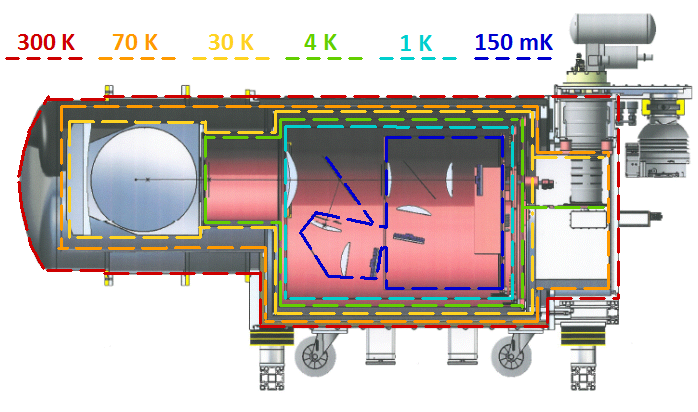
\includegraphics[width=.95\linewidth]{NIKA2_cryoStages.png}
      \caption{(Color online) Cross-section of the NIKA2 instrument illustrating the different cryogenics stages. The overall lenght of the instrument is around\,2.3 meters. The weight is close to 1300\,kg. The 150\,mK section includes the arrays, the dichroic, the polarizer and five HDPE lenses.}
         \label{Cryostat_cryo}
\end{figure}

The whole instrument includes thousands mechanical pieces, properly assembled for a total weight of around 1.3\,tons. The weight of the 150\,mK stage is of the order of 80\,kg, including few kg of HDPE (High Density PolyEthilene) low-conductance lenses. Radiation screens are placed at 1\,K (still), 4\,K (pulses tubes second stages), 30\,K and 70\,K (pulses tubes first stages).

Selected inner parts, at each stage of temperature, are coated with a high emissivity mixture of black STYCAST 2850, SiC grains and carbon powder. This coating has demonstrated its effectiveness at millimeter wavelenghts in order to suppress unwanted reflections (\cite{Calvo2010}).

Magnetic screening is added on each cryogenics stage, employing high permittivity materials down to 1K, and a pure Aluminium superconducting screen at 150\,mK enclosing the detectors. The screening is needed in order to: a) suppress the Earth magnetic field and its variations, in the instrument reference frame, during the telescope slews in azimuth; b) suppress the magnetic field variations induced by the antenna moving in elevation. 

The operation of the NIKA2 cryostat does not require cryogenic liquids, and is fully remotely controlled. The whole cool-down procedure, largely automatised, lasts about five days. Four days are required for the pre-cooling and thermalisation of the three coldest stages at around 4\,K. During the last 24 hours, the dilution procedure is started, allowing further cooling down to base temperature. Two additional days before stable observations are usually foreseen in order to ensure the perfect thermalisation of all the low-thermal-conductance optics elements like the lenses, the filters and the baffles coating. The system is designed for continuous operations and long observational runs. It has showed so far the needed stability of the base temperature over roughly one month, with no sign of degradation in performance. The stability of the detectors temperature is better than 0.1\,mK RMS over the duration of a typical observational block (scan), i.e. roughly 15\,min. This is largely within the specifications, also considering the weak sensitivity of KID detectors to variations of the base temperature. 


 \subsection{The focal plane arrays}

Each array is fabricated on a single 4 inches High Resistivity (HR) silicon wafer, on which a thin aluminium film (18\,nm) is deposited by e-gun evaporation under Ultra-High Vacuum conditions. The use of thin superconducting films has a double advantage. First, it increases the kinetic inductance of the strip, making the detectors more responsive. And second, it maximises its normal state resistivity. An almost perfect match of the LEKID meander to the free space impedance of the incoming wave is thus possible, ensuring a quantum efficiency exceeding 90\% at the peak. The NIKA2 pixels are all based on the Hilbert fractal geometry proposed some years ago by our group (\cite{Roesch2012}). 

In NIKA, we had adopted standard pixels coupled to a CoPlanar Waveguide (CPW) readout line, with bondings across the central line to suppress the spurious slotline modes. These modes are associated to a symmetry-breaking between the ground planes at each side of the line itself. To optimize the optical coupling to the incoming milimetre radiation, we had adopted a back-illumination configuration, in which the light passes through the silicon wafer before reaching the pixels. To attenuate the refraction index mismatch, we had realised a grid of perpendicular grooves at the bottom of the wafer, resulting in an effective dielectric constant which is in between vacuum and silicon (\cite{Goupy2016}). The total thickness of the silicon wafer, and the depth of the grooves, were chosen to optimize the anti-reflection effect. A superconducting lid was then set at an optimised distance behind the detectors plane, acting at the first order as a $\lambda/4$ backshort. 

The same approach was originally planned for NIKA2. During the phase of the detectors development, however, we realised the practical limitations of the CPW coupling approach, in particular considering the thousands bondings required to ensure the exclusive propagation of the CPW mode. We then decided to study and test a different kind of transmission line, the microstrip (MS). This kind of feedline only supports one propagating mode, and is thus immune from the risk of spurious modes. Furthermore, the aluminium ground plane is located on the opposite side of the wafer with respect to the detectors. This might reduce the still poorly understood residual electro-magnetic cross-coupling between resonators (pixels).

The MS propagation mode shows an electric field oscillating, in the cold HR Silicon almost perfect dielectric, between the strip line (feedline) and the underlying ground plane (see figure  \ref{CPWvsMS}). The main drawback of the MS coupling lies in the fact that it forces, at least for dual-polarisation imaging applications, front-illuminating the detectors. It is thus more adapted for relatively narrow-band (e.g. $\Delta f / f  \leq 30 \%$) applications. This is however perfectly compatible with the NIKA2 goals.  

\begin{figure}[h]
   \centering
    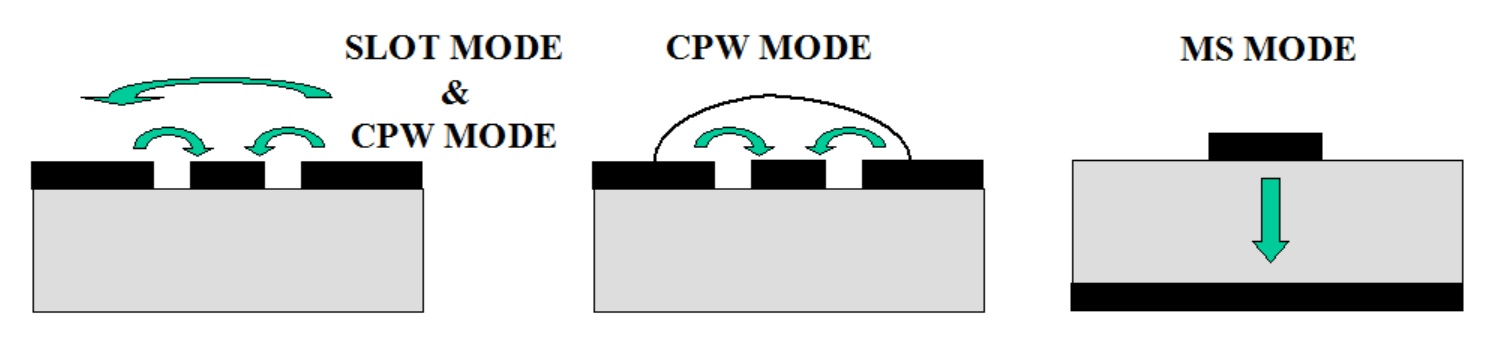
\includegraphics[width=.95\linewidth]{CPWvsMS.png}
      \caption{(Color online) In grey, the HR Silicon substrate, while in black the aluminium films are represented. Left: the CPW transmission line without across-the-line bondings, associated to strongly non-uniform performance of the detectors array. Center: the CPW with across-the-line bondings, configuration adopted in NIKA. Right: the microstrip (MS) configuration adopted in NIKA2, ensuring single-mode propagation and easiest implementation of very large arrays.}
         \label{CPWvsMS}
\end{figure}

In both cases, the distance between the pixels and the feedline is chosen in order to satisfy optimal coupling conditions. These are achieved when the coupling quality factor, $Q_c$, is of the same order as the internal quality factor $Q_i$ observed under typical loading condition. In the case of NIKA2, $Q_c\sim10,000$. A metal loop is added around each MS-coupled pixel to shield them from the feedline and achieve the wanted coupling without sacrificing the compactness of the pixels packaging (see figure \ref{Pixels}). 

In NIKA2, the 150\,GHz channel is equipped with an array of 616\,pixels, disposed to cover a circle with a 78\,mm diameter. Each pixel has a size of $2.8\times2.8\textrm{mm}^2$. This is the maximum size that can be adopted without degrading the telescope resolution, as it corresponds roughly to a $1 F \lambda$ sampling of the focal plane. The array is connected over four different readout lines, and shows resonance frequencies between 0.9 and 1.4\,GHz. The thickness of the Silicon substrate is around 150\,microns, calibrated to maximize the optical absorption at 150\,GHz. 

\begin{figure}[h]
   \centering
    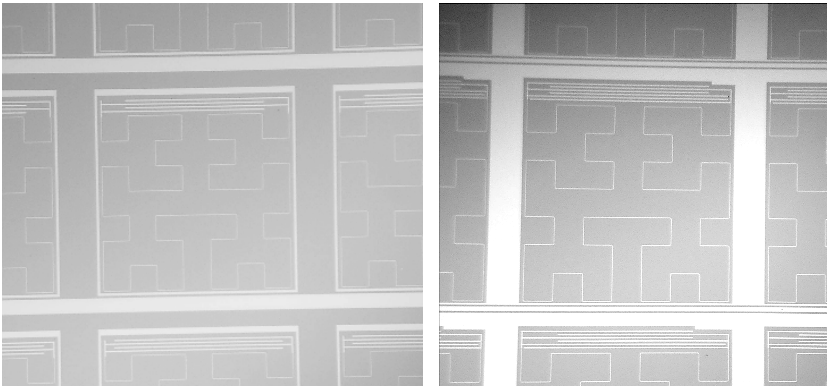
\includegraphics[width=.95\linewidth]{CPWeMS.png}
      \caption{(Color online) Left: a front-illuminated microstrip (MS) pixel for the 260\,GHz band of NIKA2. The pixels size is $2\times2\textrm{mm}^2$. Right: a back-illuminated coplanar waveguide (CPW) pixel used for the 150 GHz band in NIKA. The pixels size was in that case $2.3\times2.3\textrm{mm}^2$. Both designs are based on Hilbert-shape absorbers/inductors.}
         \label{Pixels}
\end{figure}

In the case of the 260\,GHz band detectors, the pixel size is $2\times 2\mathrm{mm}^2$, to ensure a comparable $1 F \lambda$ sampling of the focal plane. In order to fill the two 260\,GHz arrays, a total of 1140 pixels are needed in each of them. The smaller pixels dimensions compared to the 150\,GHz band lead to slightly higher resonance frequencies that are now comprised between 1.9 and 2.4\,GHz. Each of the 260\,GHz arrays is connected over eight different readout lines.  The thickness of the substrate is around 260\,microns, calibrated to maximize the optical absorption at 260\,GHz. 

\begin{figure}[h]
   \centering
    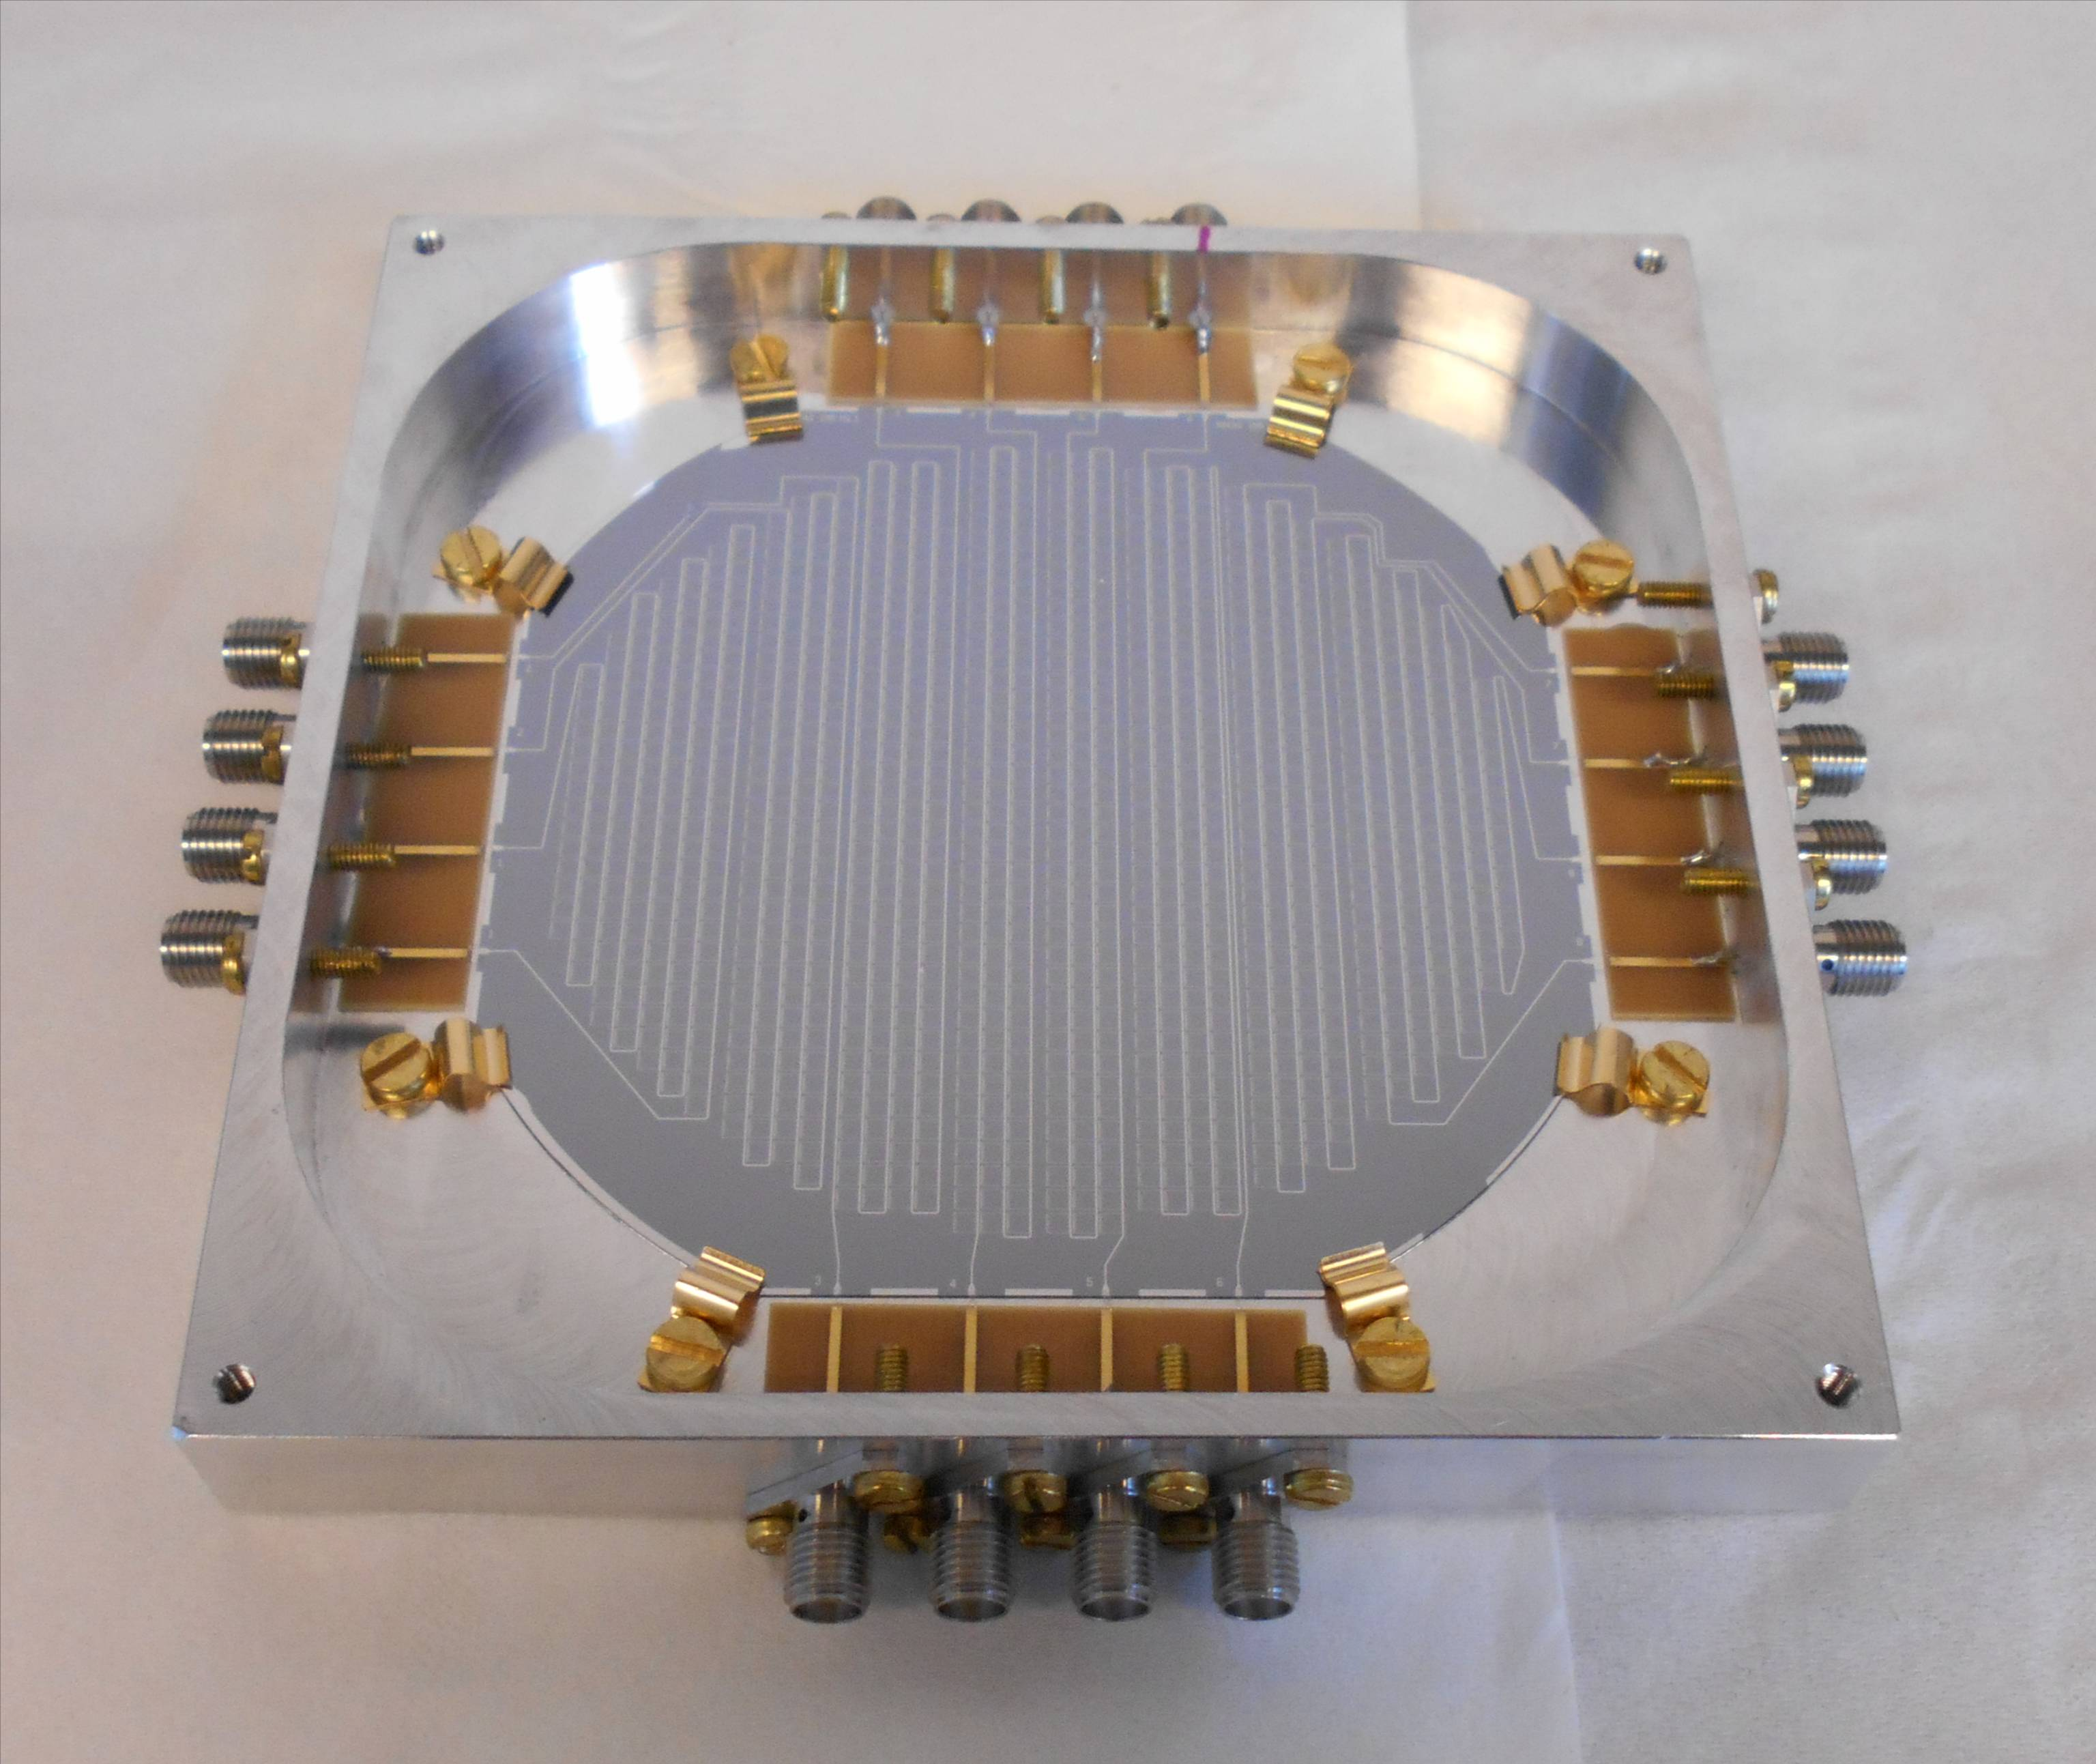
\includegraphics[width=.95\linewidth]{1mm_array.jpg}
      \caption{(Color online) One of the 260\,GHz NIKA2 arrays after packaging. The number of pixels designed for this array is 1,140.}
         \label{Array}
\end{figure}

Please refer to figure \ref{Cryostat} for an illustration of the positioning of the three arrays in the NIKA2 cryostat.
 
\begin{figure}[h]
   \centering
   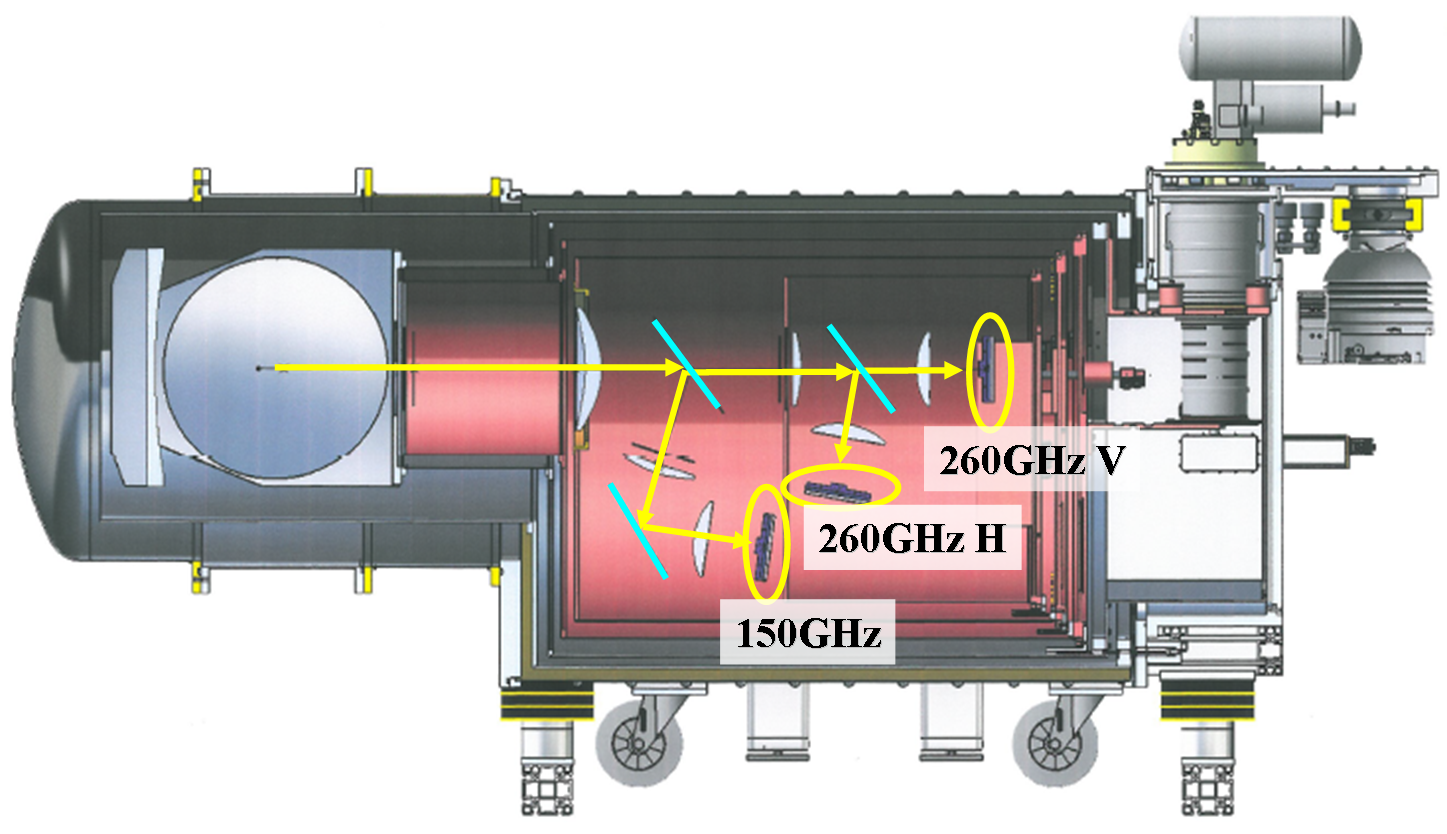
\includegraphics[width=.95\linewidth]{Fig1_cryo.png}
      \caption{(Color online) Cross-section of the NIKA2 instrument illustrating the three detectors arrays (150\,GHz, 260\,GHz-V and 260\,GHz-H). The optical axis and the photons direction of propagation is shown as well.}
         \label{Cryostat}
\end{figure}


 \subsection{The cold optics}

In this section we describe in some detail the internal (cooled) optics. More details concerning the telescope interface optics are given in par.~\ref{The integration at the telescope}.

NIKA2 is equipped with a reflective cold optics stage held at a temperature of around 30\,K. The two shaped mirrors (M7 and M8) are mounted in a specially-designed low-reflectance optical box. The stray-light suppression is further enhanced by a multi-stage baffle at 4\,K.

The refractive part of the NIKA2 cold optics is mounted at 1 K and at the base temperature. The HDPE lenses, except those placed in front of the 260\,GHz arrays, are AR-coated. The coating is realised by a specific, custom machining of the surfaces. A 30-centimeters diameter air-gap dichroic splits the 150\,GHz (reflection) from the 260\,GHz (transmission) beams. This dichroic, ensuring better flatness compared to the standard hot-pressed ones, has been developed in Cardiff specifically for NIKA2. A grid polarizer ensures then the separation of the two linear polarisations on the 260\,GHz channel. Please refer to fig.~\ref{Cryostat_optics} for a schematic cross-section of the inner optics.

\begin{figure}[h]
   \centering
   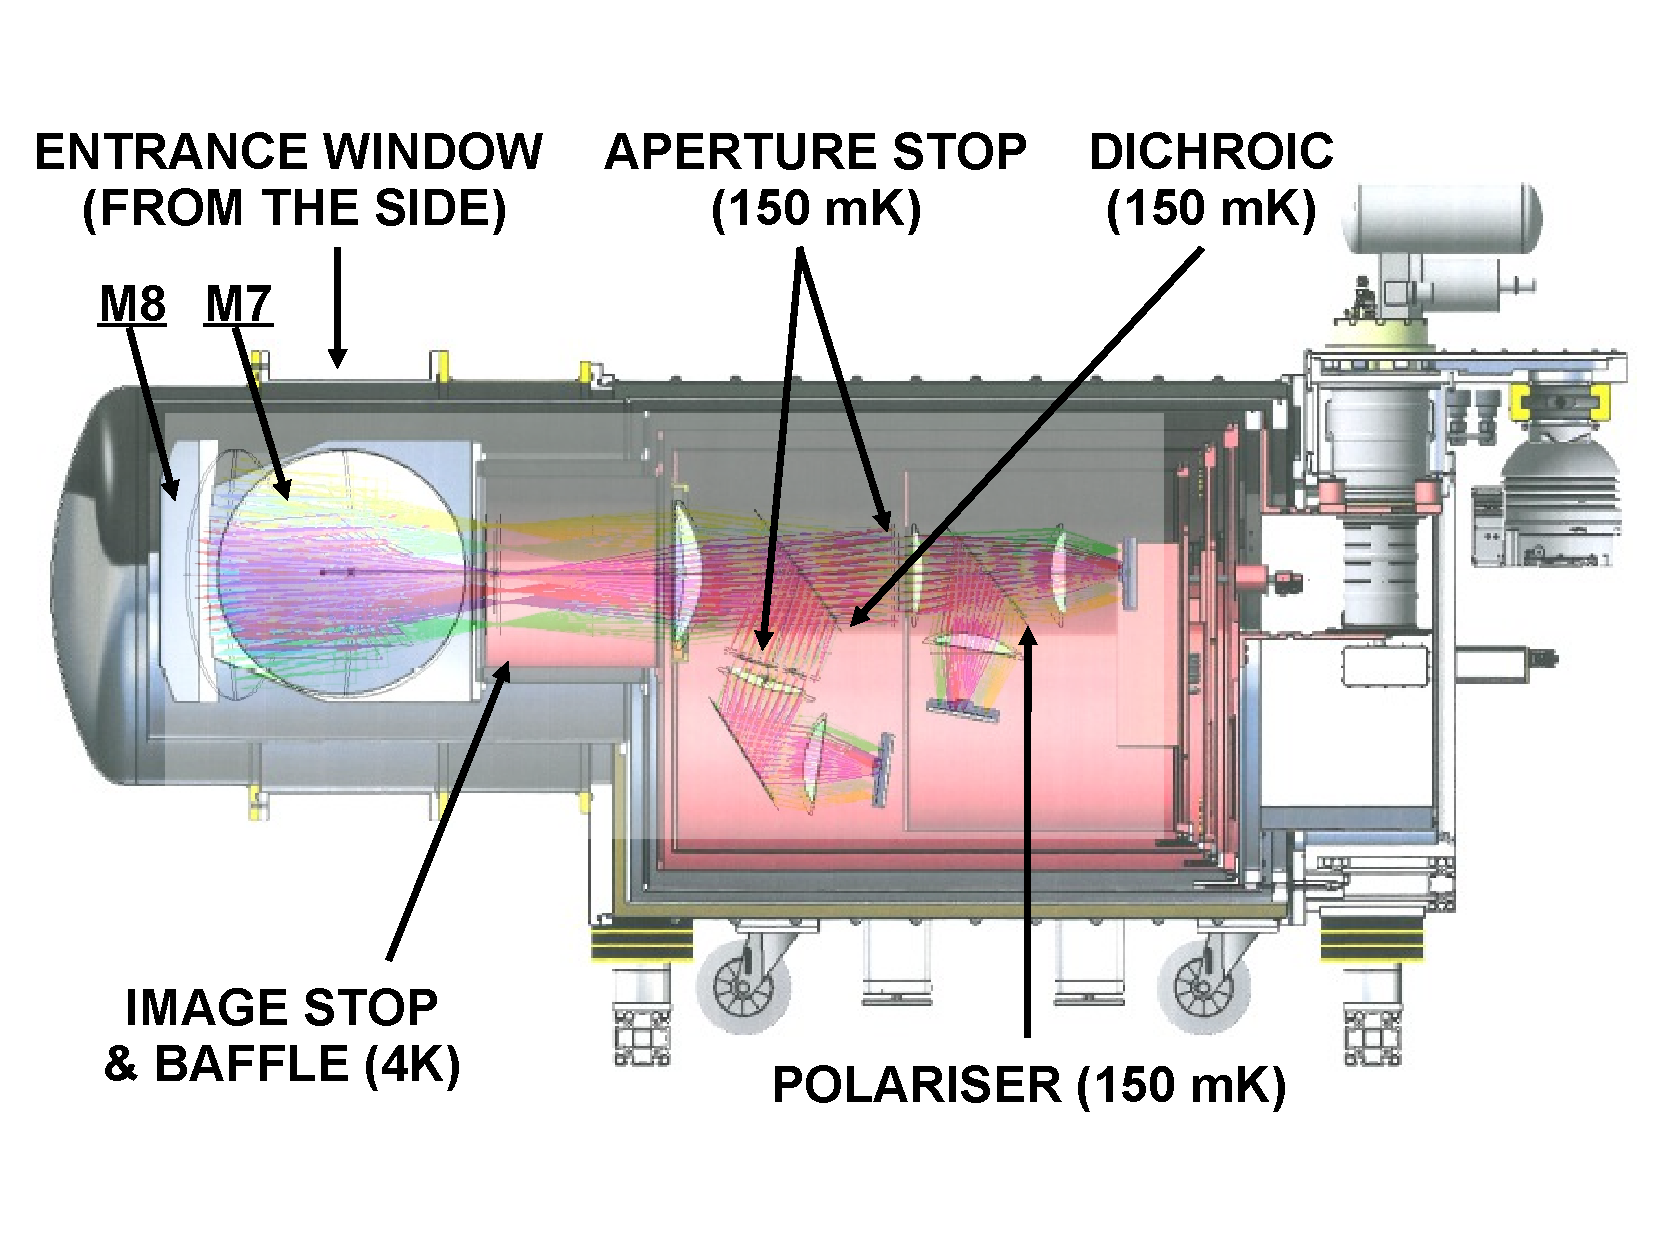
\includegraphics[width=.95\linewidth]{NIKA2_optics.pdf}
      \caption{(Color online) Cross-section of the NIKA2 instrument illustrating the cold optics and the main elements and surfaces described in the text.}
         \label{Cryostat_optics}
\end{figure}

The filtering of unwanted (off-band) radiation is provided by a suitable stack of multi-mesh filters placed at all temperature stages. In particular, three IR-cut filters are installed at 300\,K, 70\,K and 30\,K. Multi-mesh low-pass filters, with decreasing cutoff frequencies, are mounted at 30\,K, 4\,K, 1\,K and at base temperature. Band-defining filters, custom-designed, are interposed at base temperature in order to optimally match the atmospheric windows. 

%POLARISATION FACILITIES (Andrea)
To exploit the NIKA2 polarisation capabilities, a modulator is added when operating the instrument in "polarized mode". It consists of a multi-mesh hot-pressed Half-Wave-Plate (HWP) (\cite{Pisano2016}) mounted in front of the cryostat window. The modulator uses a stepping motor and is operated at mechanical frequencies of up to 3\,Hz, corresponding to 12\,Hz concerning polarisation modulation speed. In order to detect the totality of the photons, the modulated polarised signal is then projected onto the two 260\,GHz arrays by the 45 degrees wire-grid polarizer at base temperature.  


 \subsection{The readout electronics}

One of the key advantages of the KID technology is the simplicity of the {\bf{cold electronics}} installed in the cryostat.
In NIKA2, each block of around 150 detectors is instrumented by a single coaxial line providing at one end the excitation, and the readout at the other end. The excitation lines, composed of stainless steel cables, are running from 300\,K down to sub-Kelvin temperature. They are properly thermalised at each cryostat stage, and a fixed attenuation of 20\,dB is applied at 4\,K in order to suppress the room temperature thermal noise. Each excitation line ends in an SMA connector (EXCitation input) and an ad-hoc launcher connected, through superconducting (Aluminium) microbondings, to the silicon wafer holding the detectors. The approximate excitation power per resonator is usually of the order of 10\,pW.

On the readout side, the same types of microbondings are used to transfer the signal out of the focal plane and to make it available on a second SMA connector (MEASurement output). Then a superconducting (Nb) coaxial cable is used to connect directly the measurement output to the input of a low-noise cryogenics amplifier (LNA). The amplified signal provided by the LNA is transfered through the remaining cryostat stages (up to 300\,K) via stainless steel cables. 
The LNA, which operate at frequencies up to 2.5\,GHz, show noise temperatures comprised between 2\,K and 5\,K and are held at a physical temperature of about 8\,K. That means that the input amplifier noise is equivalent to the thermal Johnson noise of a 50-Ohms load held at 2-5\,K.

The cryogenics amplifiers used by NIKA2 have been developed, fabricated and tested at the Yebes observatory and TTI Norte company, both located in Spain. The specifications of the amplifiers have been elaborated by the NIKA2 group.

NIKA2 is composed by a total of about 2,900 pixels and is equipped with twenty feed-lines. Thus, it employs twenty cryogenics amplifiers (four for the 150\,GHz array and eight for each of the 260\,GHz arrays). The polarisation of the LNA stages is provided by a custom electronics box remotely controlled and allowing the optimizations of the biases according to the slightly different characteristics of the front-end high electrons mobility transistors (HEMT). 

\begin{figure}
\begin{center}
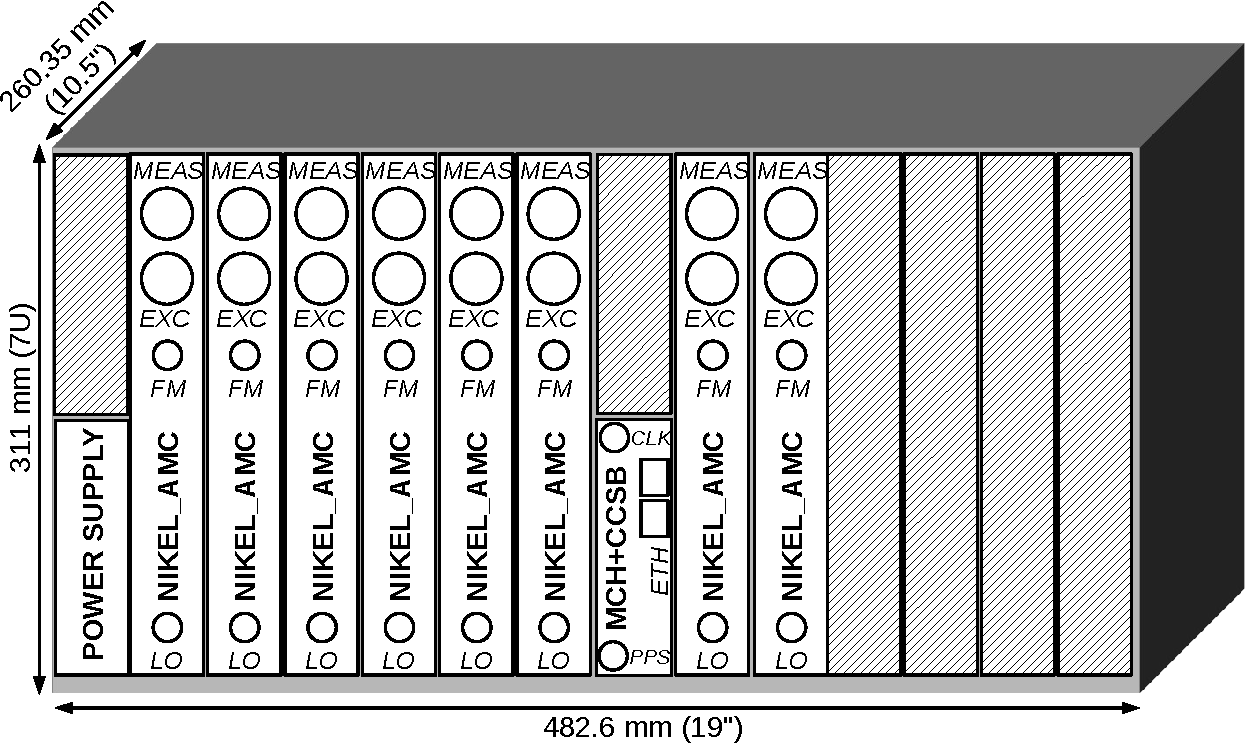
\includegraphics[angle=-90,width=0.45\textwidth]{NIKA_crate}
\caption{Overview of one array readout electronics crate.
It is equipped with 4 (or 8) readout boards lodged in Advanced Mezzanine Card slots (NIKEL\_AMC), one central and clocking and synchronization board (CCSB) mounted on the MicroTCA Carrier Hub (MCH) and one 600\,W power supply.
The crate allocated to the 150\,GHz channel uses 4 NIKEL\_AMC while the others use 8 NIKEL\_AMC boards.
\label{crateFig}}
\end{center}
\end{figure}

The \textbf{warm electronics} required to digitize and process the 2,900 pixels signals was specifically designed for that purpose.
It is composed of twenty readout cards (one by feed-line) named New Iram Kid ELectronic in Advanced Mezzanine Card format (NIKEL\_AMC).
As shown in fig.~\ref{crateFig}, the cards are distributed in three micro-Telecommunication Computing Architecture (MTCA) crates.
A central module, composed of a commercially available Mezzanine Control Hub (MCH) and of custom made mezzanine boards, is used to distribute a Rubidium reference clock (CLK) and a pulse per second (PPS) provided by GPS receiver and to control the crate.
This electronics is fully described in previous papers (\cite{Bourrion2012,Bourrion2016}).

In summary, the NIKEL\_AMC is composed of two parts: the radio-frequency (RF) part and the digitization and processing section.
The integrated RF part ensure the transition from and to the baseband part.
It uses the local oscillator (LO) input to perform up and down-conversions.
To instrument the 150\,GHz array (resonances from 0.9\,GHz to 1.4\,GHz) and the 260\,GHz arrays (resonances from 1.9\,GHz to 2.4\,GHz), the used LO input frequency are respectively 0.9\,GHz and 1.9\,GHz. The digitization and signal processing part, which is done at baseband, relies on channelized Digital Down Conversion (DDC) and their associated digital sine and cosine signal generators to build the excitation signal and to process the down-converted measurement signal.
The processing heavily relies on Field Programmable Gate Arrays (FPGA) while the interfacing to and from the analog domain is achieved by 1\,GSPS Analog to Digital and Digital to Analog Converters (ADC and DAC).
Finally, the electronics covers a bandwidth of 500\,MHz and can instrument up to 400\,KID in this bandwidth. In NIKA2 about 150 KID per board are instrumented, leaving room for placing a number of dark (off-resonance) excitation tones, and allow future developments of the instrument. 

It must be noted that for implementation reasons (\cite{Bourrion2012,Bourrion2016}) the excitation signal, nominally covering 500\,MHz is constructed by five DAC, each spanning 100\,MHz.



\subsection{Laboratory tests}
\label{Laboratory tests}

The NIKA2 arrays have been pre-characterised in laboratory under realistic illumination conditions. In order to compensate the absence of the telescope optics, we have added an additional lens at the cryostat input window. This lens is creating an image of the focal planes onto our "sky simulator", described in previous papers (\cite{Catalano2014}, \cite{Monfardini2011}). A warm source, moved in front of the sky simulator by means of an x-y stage, allows beams shape and arrays geometry (e.g. pixel-per-pixel pointing) characterisations. The sensitivity is calculated by excecuting calibrated temperature sweeps of the sky simulator, and measuring the signal-to-noise ratio of the detected signal. A photometric model has been elaborated, based on ray-tracing simulations and assuming reasonable overall optics (filters, lenses) transmission. In particular, the overall transmission of the instrument, mainly determined by the lenses and the filters, lies around 35\%. On top of that, the quantum efficiency of the detectors, integrated in the band of interest, is comprised between 60\% (260\,GHz arrays) and 80\% (150\,GHz array). The frequency sweep of the four lines making up to 150\,GHz array are shown in figure \ref{VNA}. The average number of identified resonances over the twenty feedlines exceeds 90\% when compared to the number of pixels implemented by design. For example, in the case of the 150\,GHz array at least 580 beams are identified during laboratory tests, amounting more than 94\% of the total 616 implemented in the design. 

\begin{figure}[h]
\begin{center}
   \centering
    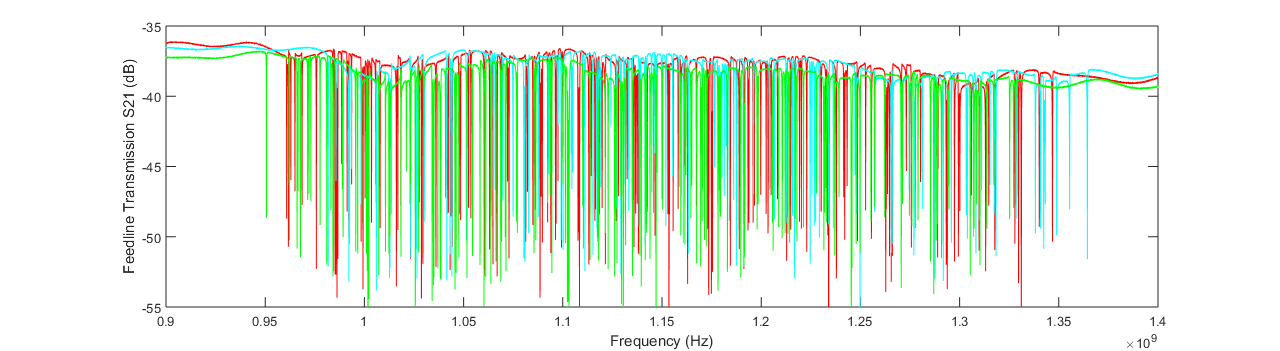
\includegraphics[width=1.05\linewidth]{VNA_scans_150GHz.png}
    \caption{(Color online) Resonances sweep for the four feedlines of the 150\,GHz array. The lines 1,2,3,4 are respectively shown in blue, red, cyan and green. The y-axis represents the transmission of the feedline (parameter S21) and is expressed in dB. Each dip correcponds to a resonance/pixel. About 94\% of the pixels are identified with a resonance and are sensitive to light.}
         \label{VNA}
\end{center}
\end{figure}

The measurable quantity, proportional to the incoming power per pixel, is the shift in frequency of each resonance (pixel) (\cite{Swenson2010}). That's why our noise spectral densities are expressed in Hz/Hz$^{0.5}$, and the responsivities are given in kHz/K. By sweeping the temperature of the sky simulator, we have estimated average responsivities around 1 and 2\,kHz/K at respectively 150 and 260\,GHz. The average frequency noise levels, for the two bands, are on average about 1 and 3\,Hz/Hz$^{0.5}$, resulting in NET (Noise Equivalent Temperature) of the order of 1 and 1.5\,mK/Hz$^{0.5}$ per pixel at 150 and 260\,GHz respectively. These figures are calculated at a representative sampling frequency of 5\,Hz. 

\begin{figure}[h]
\begin{center}
   \centering
    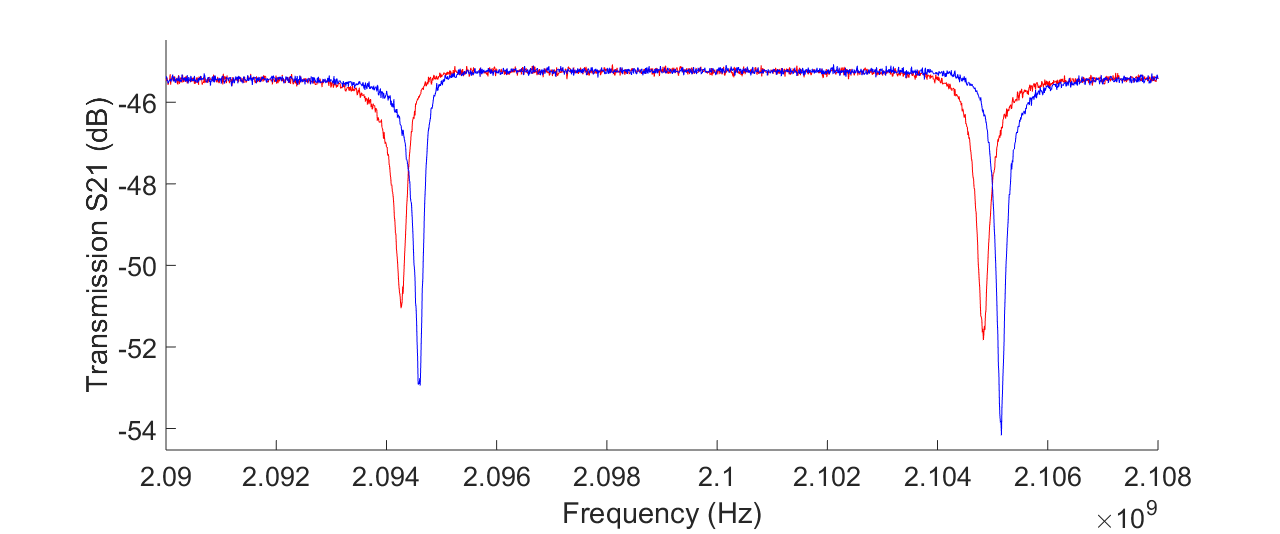
\includegraphics[width=1.05\linewidth]{Shift_f_260GHz.png}
    \caption{(Color online) Responsivity estimation using the sky simulator. We illustrate two typical resonances, plotting the S21 transmission parameter against frequency. Blue line: cold sky simulator ($T_{SS} \sim 100\,K$). Red line: 300K background. The measured average responsivity, i.e. the shift in frequency per unit temperature background variation, is around 2\,KHz for the 260\,GHz arrays and 1\,KHz/K in the case of the 150\,GHz.}
         \label{Shift_f}
\end{center}
\end{figure}

These figures are in line with the expectations. An example of Sky Simulator testing, allowing the measurement of the responsivity, is reported in figure \ref{Shift_f}. Noise spectra has been acquired as well in laboratory, with results then fully confirmed at the telescope, with NIKA2 observing the real Sky. Please refer to the paragraph \ref{Noise and sensitivity} for a more detailed discussion concerning the noise properties. 


The spectral characterisation of the arrays and the overall optical chain of NIKA2 has been achieved using a Martin-Puplett Interferometer (MpI) built in-house (\cite{Durand2008}) and specifically dedicated to instruments characterisation. The two arrays operating at 260\,GHz, mapping different polarisations, exhibit a slightly different spectral behaviour probably due to a tiny difference in the silicon wafer and/or Aluminium film thicknesses. The observed shift of the central frequency (265\,GHz for the V array versus 258\,GHz of the H) can be explained by about 5\,microns change in the substrate thickness.

\begin{figure}[h]
   \centering
%    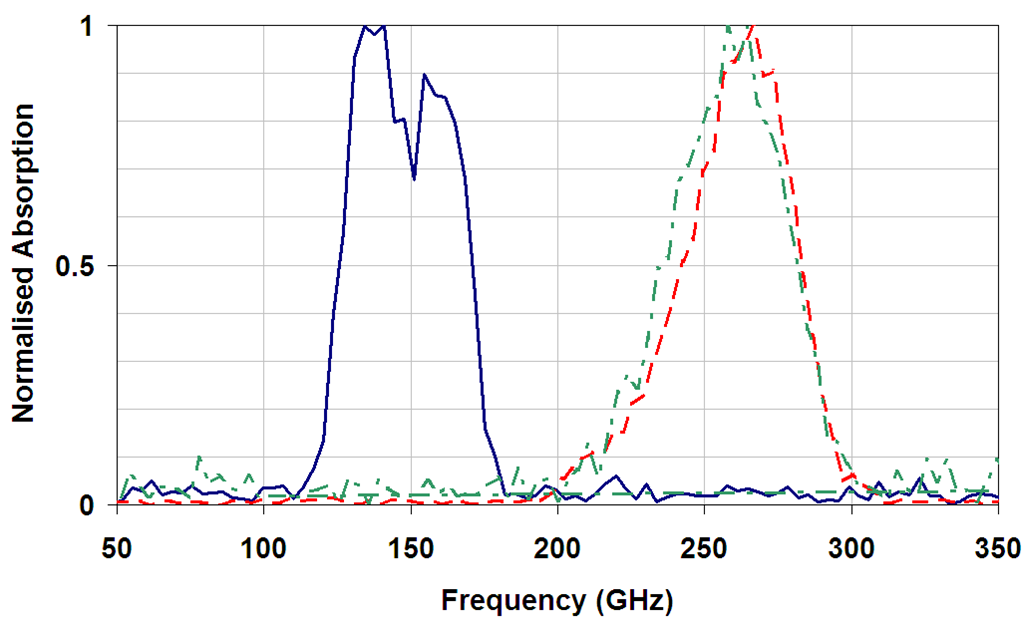
\includegraphics[width=0.9\linewidth]{Fig4_spectra.png}
    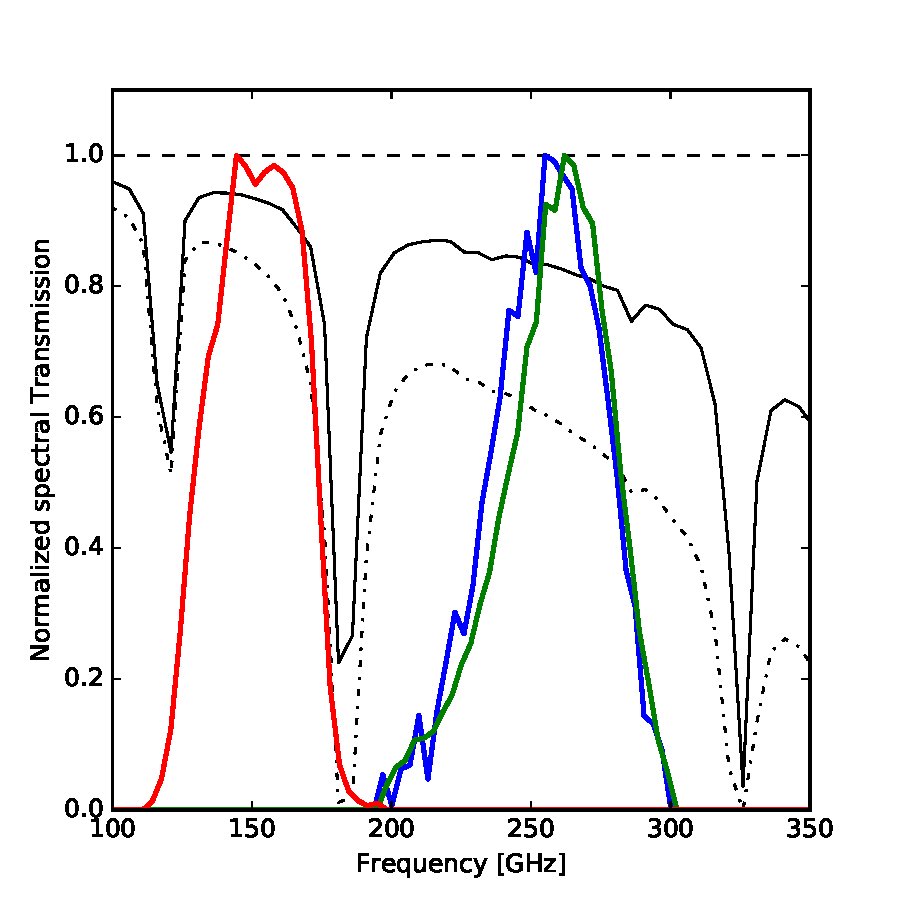
\includegraphics[width=0.9\linewidth]{atm_transmission.pdf}
      \caption{(Color online) NIKA2 spectral characerisation. Solid line (blue): 150 GHz array, FWHM: 126-170 GHz; dashed line (red): 260 GHz V, FWHM: 242-283 GHz; dashed-dotted line (green): 260 GHz V, FWHM: 235-281 GHz.}
         \label{Fig4}
\end{figure}

The sky simulator allowed also a rough but crucial estimation of the parasitic radiation. By comparing measures acquired at several simulator distances with respect to the cryostat window, we fit an equivalent 15\,K additional focal plane background due to the ambient temperature stray radiation. This is lower than the very best equivalent Sky temperature at Pico Veleta ($\approx 20\,K$), and confirms that NIKA2 is not affected by this effect. In comparison, in NIKA we had estimated around 35\,K additional background, slighly limiting the performance in that case. 

In summary, the overall performance of the instrument, mesured preliminarily in laboratory, is in line with the NIKA2 specifications, paving the way for the installation at the telescope described briefly in the next paragraph. 

\subsection{The integration at the telescope}
\label{The integration at the telescope}

NIKA2 has been transported in pieces from the integration hall in Grenoble to the observatory on the end of September, 2015. Successful installation of the instrument took place in early October 2015 at the IRAM 30-meters telescope on Pico Veleta (Sierra Nevada, Spain). To prepare for this installation, the optics of the receiver cabin (M3, M4, M5 and M6) had been modified earlier in 2015 in order to allow increasing the telescope field-of-view up to the 6.5\,arc-min covered by NIKA2. M3 is the Nasmyth mirror attached to the telescope elevation axis. M4 is a flat mirror that can be turned manually in order to feed the beam either to NIKA2 or to the etherodyne spectroscopic instruments. The M5 and M6 non-flat mirrors are dedicated to the NIKA2 camera. 

\begin{figure}[h]
   \centering
    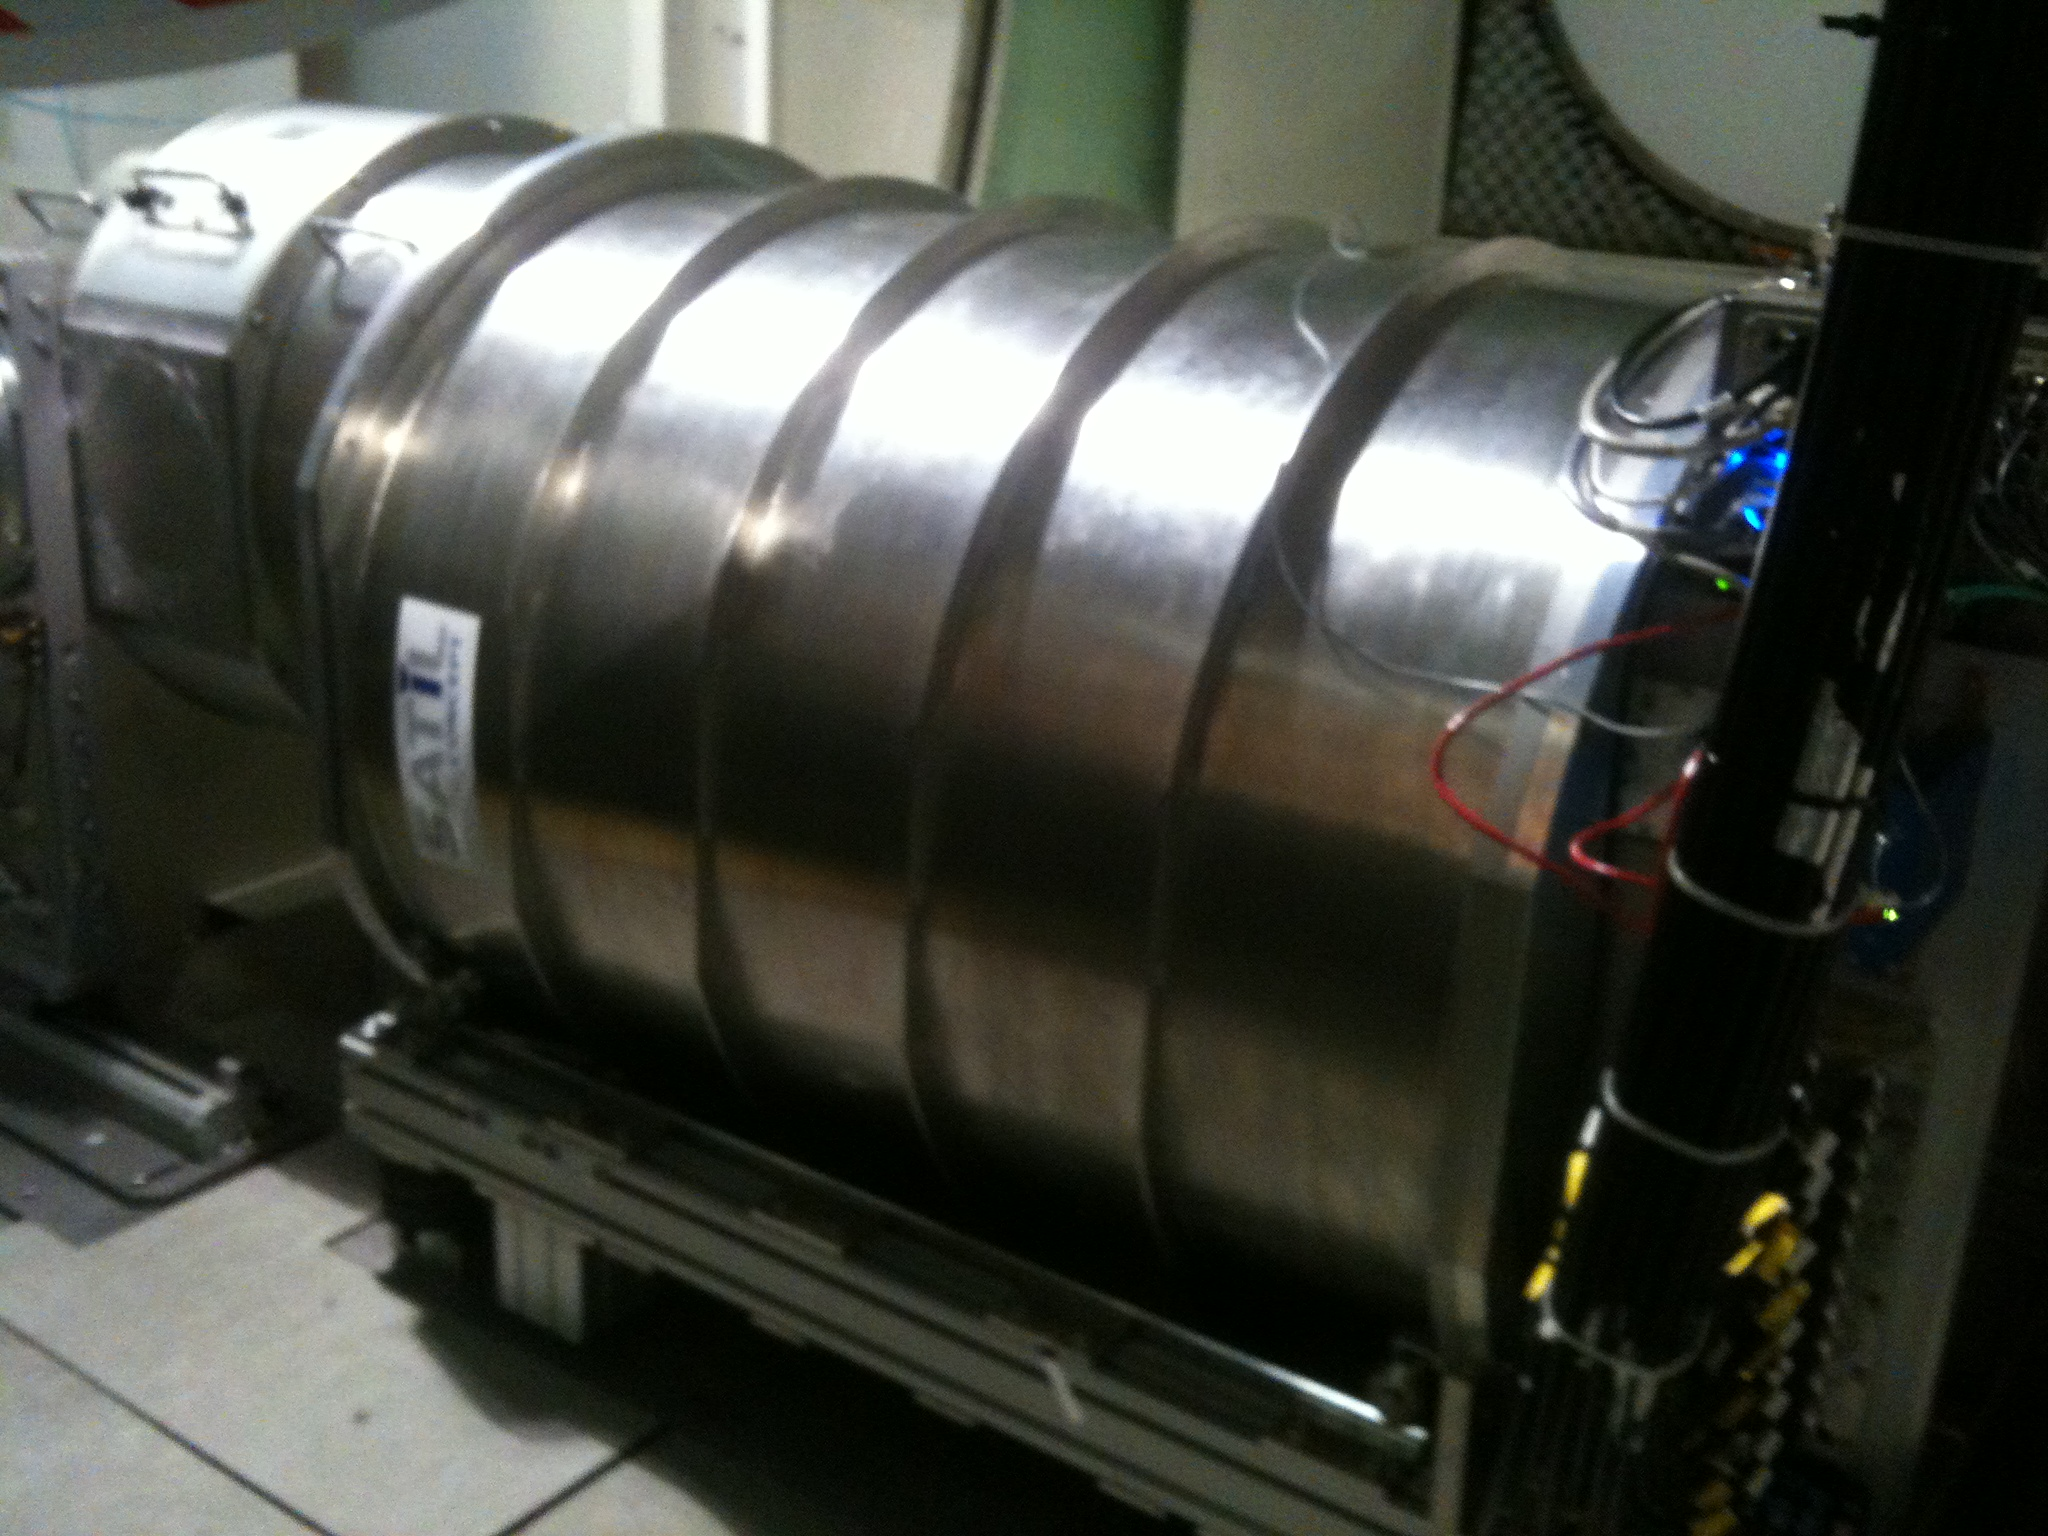
\includegraphics[width=.85\linewidth]{NIKA2cryo.jpg}
      \caption{(Color online) A picture of the NIKA2 cryostat installed in the 30-meters telescope receivers cabin end of September, 2015.}
         \label{Fig5}
\end{figure}

The whole installation, including the cabling of the instrument, was completed in around three days. The pulse-tubes pipes, 60-meters long, run through a derotator stage in order to connect the heads in the receiver cabin (rotating in azimuth) and the compressors located in the telescope basement (fixed). A single 1 Giga-bit ethernet cable ensures the communication to and from the NIKA2 instrument and the control room. The fourty radio-frequency connections (twenty excitation lines, twenty readouts) between the NIKEL\_AMC electronics and the cryostat, on the other side of the receivers cabin, are realised using 10-meters long coaxial cables. 

The optical alignment between the instrument and the cabin optics has been achieved using two red lasers. The first was set shooting perpendicularly from the center of the NIKA2 input window, through the telescope optics and reaching the vertex. The second laser is mounted on the telescope elevation axis, reaching then, through the M4, M5 and M6 mirrors, the NIKA2 window. In both cases, we have adjusted the cryostat position and tilt to achieve good alignment. NIKA2 is equipped with an automatic system of pneumatic actuators and position detectors able to adjust the cryostat height and tilt and keep it stable. 

The first cryostat cooldown started immediately afterwards, and was achieved on October, 7th, 2015 after the nominal four days dedicated to pre-cooling and less than 24 hours during which the helium isotopes mixture is condensed in the so-called "mixing chamber" and the dilution process is started. The first technical tests demonstrated immediately that all the detectors were functional and exhibited responsivity and noise in line with the laboratory measurements presented in the previous paragraph. The first commissioning run could then start.


%______________________________________________________________



\section{The calibration procedures}

The photometry is reconstructed down to the required level thanks to three distinct procedures applied by default. First, we have implemented an electrical calibration acting directly on the KID and specific to NIKA and NIKA2 (par.~\ref{Internal detectors calibration}). Secondly, we measure, as any other instrument, a flat-field using known sources (par.~\ref{On-sky calibration}). Lastly, the atmosphere opacity correction is calculated in real time thanks to the large dynamics and linearity of the detectors (par.~\ref{Atmospheric attenuation correction}).



\subsection{Internal detectors calibration}
\label{Internal detectors calibration}
When radiation is absorbed in a KID, it breaks part of the superconducting carriers (Cooper Pairs) and creates an excess of unbound electrons (quasi-particles). This changes the impedance of the film and shifts the resonance frequency $f_0$ of the illuminated KID to lower values.
%[For small variations of the absorbed power, delta f_0 is directly proportional to $\delta P$.] 
The standard way to readout a pixel is to excite it with a tone at $f_0$ and to monitor how the In-phase ($I$) and in-Quadrature ($Q$) components of the transmitted signal are modified by the changes in $f_0$. For NIKA2 we adopted a different strategy, already developed for NIKA. Instead of using an excitation at a fixed frequency, we rapidly modulate between two different readout tones, $f^+$ and $f^-$, just above and just below $f_0$. The tones are separated by $df=f^+-f^-$. This modulation technique allows to measure, for every acquired data sample, both the values of $I$ and $Q$ and the variation $dI$, $dQ$ that is induced by the chosen frequency shift $df$. When the optical power on the detectors changes by an amount $\Delta P_{opt}$, a variation $\Delta I$, $\Delta Q$ is observed between successive data samples. The $dI$, $dQ$ values can then be used as a calibration factor to associate to the observed $\Delta I$, $\Delta Q$ the corresponding change in the resonance frequency $\Delta f_0$, and thus measure $\Delta P_{opt}$. More details on the modulated readout technique can be found in \cite{Calvo2013} and \cite{Catalano2014}.

The advantage of this solution is that the $dI$, $dQ$ values are evaluated for every data sample. If the load on the detectors change (e.g. due to variations in the atmospheric opacity), the exact shape of the resonance feature of each pixel will change, but since the calibration factor $dI$, $dQ$ is updated in real time it will take this effect into account. Its use thus strongly increases the photometric accuracy of the instrument.

Furthermore, knowing both the $I$, $Q$ and the $dI$, $dQ$ values we can also estimate the current position of a KID resonance with respect to the position of the corresponding excitation tone. In the ideal situation, these two positions should coincide. In reality, changes in the background load can make the resonances drift by a large amount. Thanks to the modulated readout, when this happens the excitation tones can be rapidly re-tuned to keep track of the new resonance positions. This tuning procedure allows us to always readout the KID with optimally placed tones, which prevent any degradation in the sensitivity of the detectors.


\subsection{Atmospheric attenuation correction}
\label{Atmospheric attenuation correction}

\begin{figure}
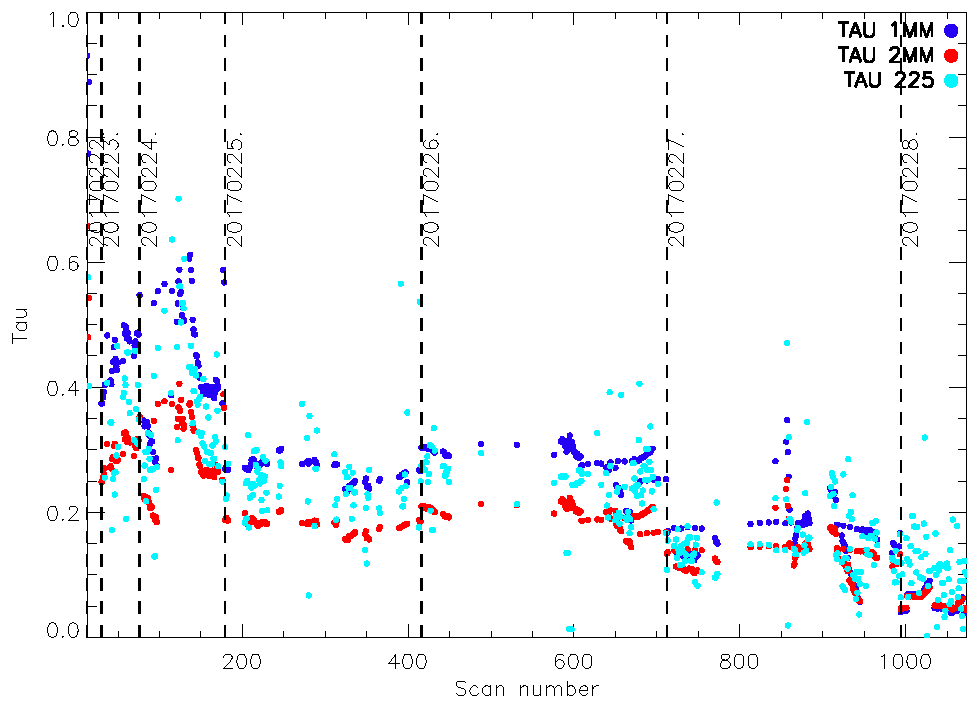
\includegraphics[scale=0.6]{./opacity_evol_run22.pdf}
\caption{Atmospheric opacity as measured from the IRAM 225~GHz taumeter (cyan), and from the NIKA2 data at 150 (red) and 260 GHz (blue) during the February NIKA2 commissioning campaign. \label{fig:taumeas}}
\end{figure}

The sky maps are corrected for the atmospheric contribution rescaling the observed signal by what that would be obtained in the absence of atmosphere. The corrected brightness is:

\begin{equation}
S^{Star} =  S^{Ground} \cdot e^{ x \tau_{scan}}.
\end{equation}

Where $\tau_{scan}$ is the opacity of the atmosphere and $x$ corresponds to the airmass at the elevation of the considered map\footnote{The airmass is the volume of air defined by its temperature and water vapor content. By assuming a homogeneous plane-parallel atmosphere, the relation between the airmass and the elevation of the telescope becomes $x = sec(\delta)$, where $\delta$ is the average elevation.}.
In NIKA2, the opacity is measured via the elevation scan technique (skydip). This procedure was successfully tested in the NIKA pathfinder producing a low-level dispersion of the derived opacity at different elevations. The details of this technique and its agreement with the Atmospheric Transmission at Microwaves (ATM) model \cite{2001IEEE....49.1683C} are described in \cite{Catalano2014}. Briefly, the underlying idea is to replace the opacity delivered by the resident IRAM tau-meter that performs elevation scans continuously at a fixed azimuth at 225~GHz, with a direct measurement that uses the NIKA2 instrument itself as a tau-meter. Using this procedure we can directly derive an opacity integrated in the NIKA2 bandpasses and at the same position of the source in the considered map. 
During a skydip, the telescope performs ten elevation steps from 19 to 65 degrees. For each step we acquire about twenty seconds of useful signal. The relation between the resonance frequency of each pixel and the airmass is given by the following equation:

\begin{equation}\label{eq:skydip}
S^{Ground}_{skydip} = C_0 + C_1 T_{atm}[1 - e^{- x \tau_{skydip}}].
\end{equation}

Where $F^{Ground}_{skydip}$ is the acquired signal which corresponds to the
absolute value of the shift in the resonance frequency for each pixel, $C_0$ is the
instrumental offset corresponding to the resonance frequency for the
considered pixel at zero opacity, $C_1$ is the calibration conversion factor in
$\mathrm{Hz/K}$, $T_{atm}$ is the equivalent temperature of the
atmosphere, $\tau_{skydip}$ is the sky opacity during the skydip, and $x$ is the airmass.

A skydip shows that the value of $tau$ is common between pixels of the same channel as expected. Coefficients  $C_0$, $C_1$ depend on the response of the detectors. Since the non-linearities of the KID frequency signal are negligible in the considered range of backgrounds, the coefficients can be applied to all the observing campaign to recover the opacity of the considered scan. This is
obtained by inverting Eq \ref{eq:skydip} on the considered map. In Fig.~??? we present the evolution of the opacities for several map of the NIKA2 commissioning  in February-March 2016 compared to the IRAM tau-meter.

%______________________________________________________________

\section{Observations and performance}
\label{Observations and performance}

The first astronomical light has been achieved in October 2015. A first technical run followed immediately. A number of commissioning runs have then been carried out between November, 2015 and April, 2017. In this paragraph we summarize the main results obtained, and allowing a good characterisation of the instrument performance. We stress however that the experience in the utilisation of NIKA2 by esternal astronomers might led in the best case to further optimisation of the instrument performances. The experience that will be accumulated in the future will eventually allow to point subtle problems that have not been evidenced during the commissioning. 

\subsection{Focal plane reconstruction}

\begin{figure*}[h]
   \centering
%    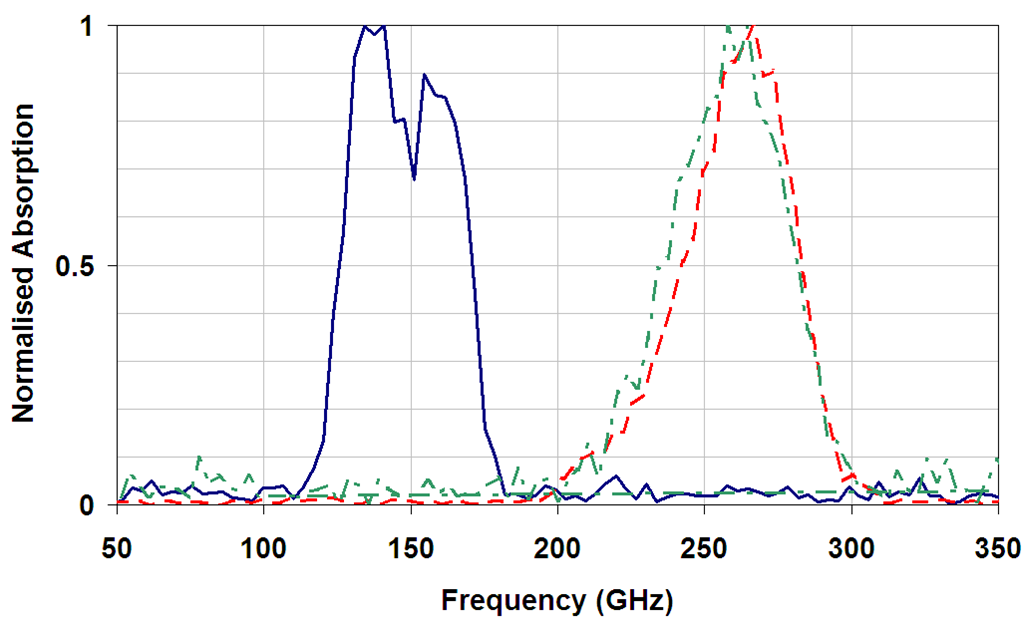
\includegraphics[width=0.9\linewidth]{Fig4_spectra.png}
    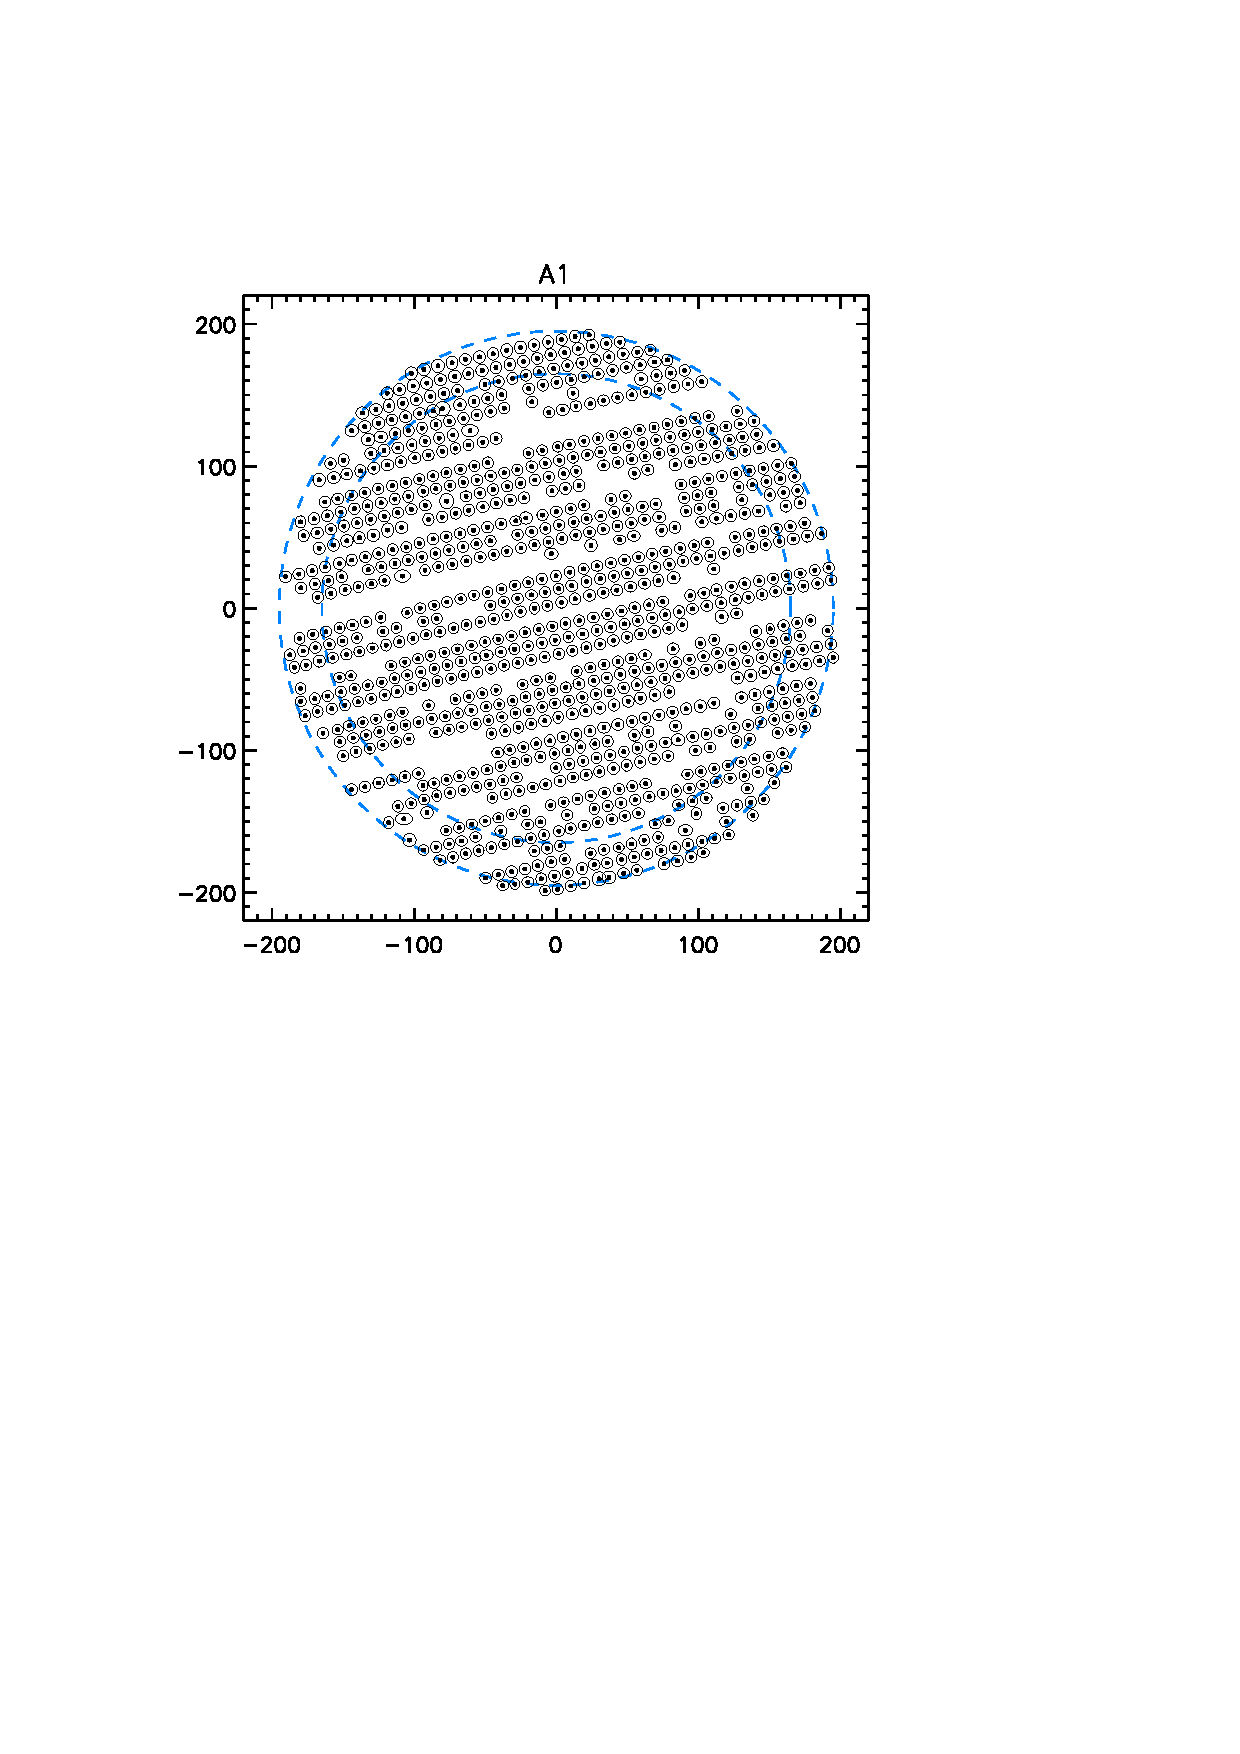
\includegraphics[trim=2cm 14cm 5cm 4cm, clip=true,width=0.33\linewidth]{A1_fwhm_valid.pdf}
   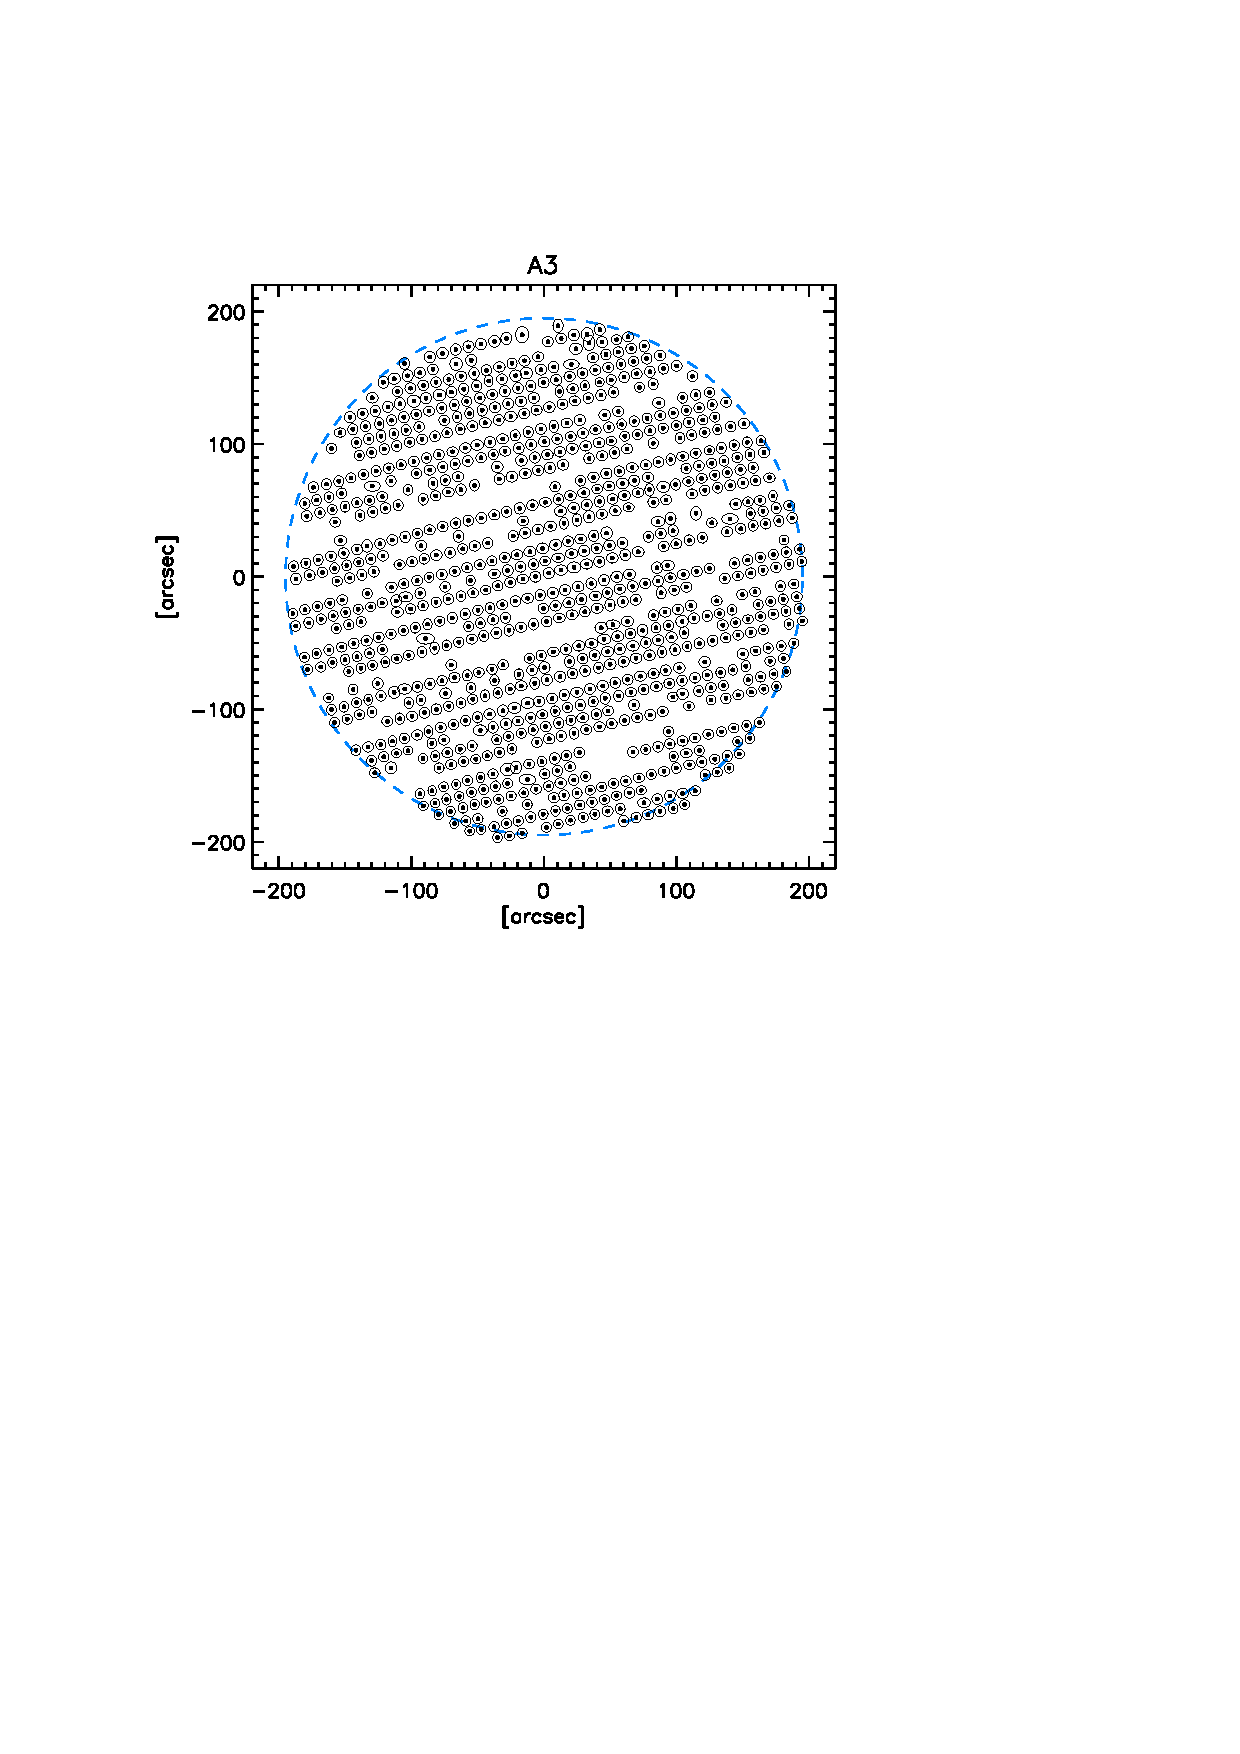
\includegraphics[trim=2cm 14cm 5cm 4cm, clip=true,width=0.33\linewidth]{A3_fwhm_valid.pdf}
   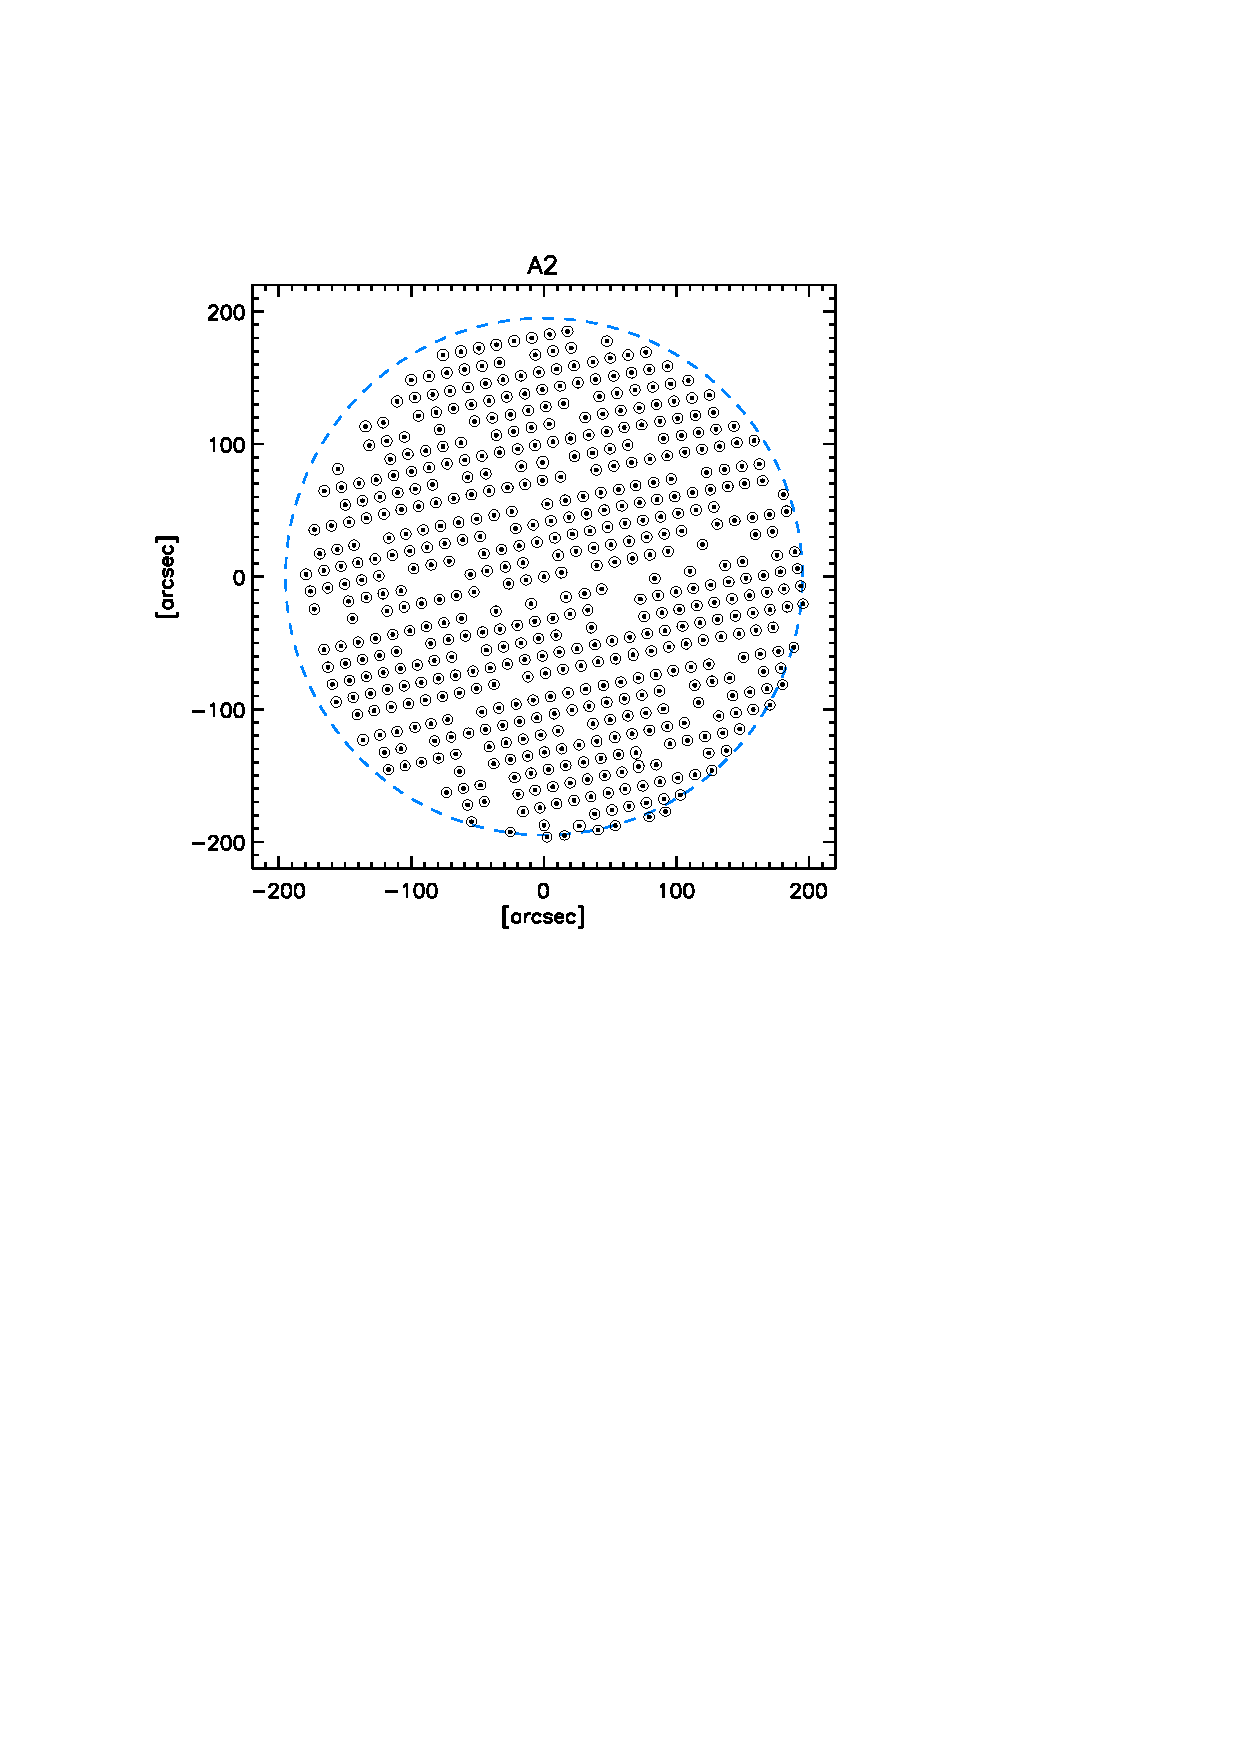
\includegraphics[trim=2cm 14cm 5cm 4cm, clip=true,width=0.33\linewidth]{A2_fwhm_valid.pdf}
       
      \caption{From left to right, detectors positions for arrays A1, A3, and A2. The three plots show the detectors that have seen the sky and passed the quality criteria for at least two focal plane reconstructions during Run10 (901, 903, 533 for A1, A3 and A2, respectively).}
         \label{fig:focalplane}
\end{figure*}

Figure~\ref{fig:focalplane} shows the position of the array A1, A3 and A2 detectors in the NIKA2 FOV. For each detector the ellipse symbol size and ellipticity
are proportional to the main beam FWHM and the ellipticity of the full beam assuming a 2D Gaussian. 

\begin{figure*}[h]
  \centering
  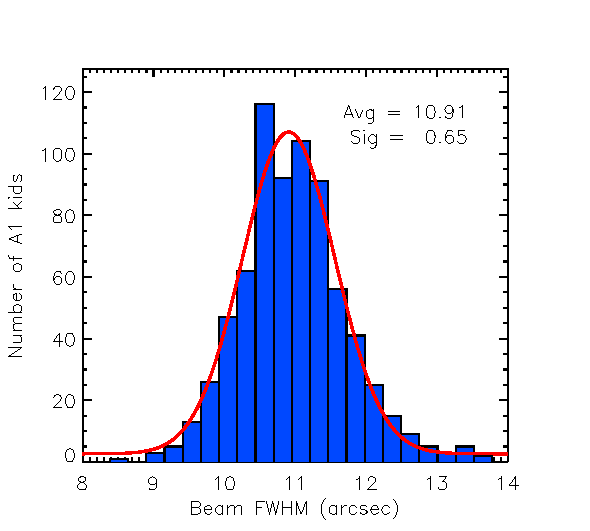
\includegraphics[clip=true,width=0.33\linewidth]{plot_histo_A1_fwhm_20170424s123.pdf}
  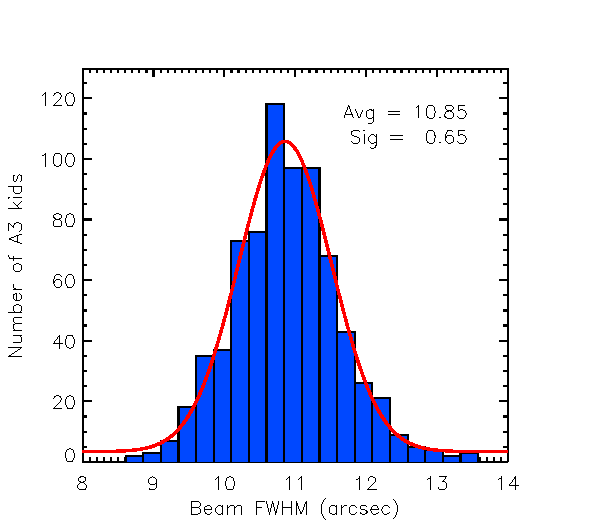
\includegraphics[clip=true,width=0.33\linewidth]{plot_histo_A3_fwhm_20170424s123.pdf}
  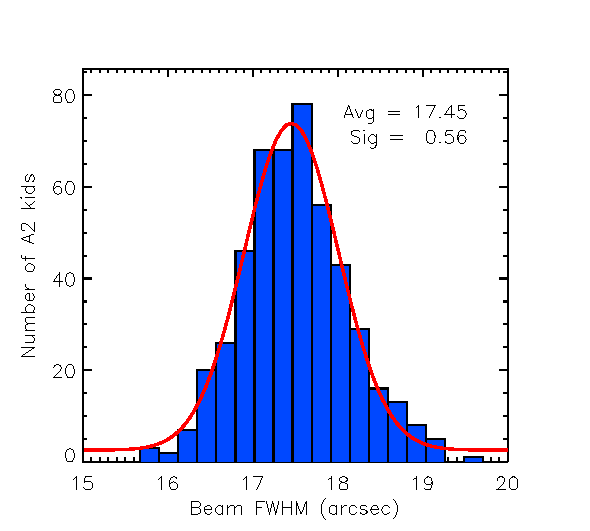
\includegraphics[clip=true,width=0.33\linewidth]{plot_histo_A2_fwhm_20170424s123.pdf}
  
\caption{From left to right, main beam FWHM distribution for arrays A1, A3, and A2 detectors. The main beam FWHM is the geometrical combination of the two-orthogonal FWHM estimates obtained from an elliptical Gaussian fit on side-lobe masked individual maps per KID (see text). The red curves show the Gaussian fit on the histogram, which provide averaged main beam FWHM of $10.9\arcsec$ at $260~\rm{GHz}$ and $17.5\arcsec$ at $150~\rm{GHz}$ in agreement with the main beam estimates from the deep beam map presented in Fig.~\ref{fig:beampattern}. The dispersion of about $0.6\arcsec$ is expected and partly due to slight change of the focus across NIKA2 FOV (of the order of -0.2~\rm{mm} at two arcmin from the FOV center).}
  \label{fig:focalplane_histo}
\end{figure*}

[LP]
Individual beams per KID across NIKA2 FOV are characterised in using
deep-integrated raster-scan observation, referred to as beam-map scan, of bright point-like
astronomical sources to project $4~\arcsec$ resolution individual maps
per KID. To isolate the main beam contribution to the total beam, the
side lodes are masked out using annulus masks centered on the peak
signal, of $50\arcsec$ external radius and of internal radius of
$9\arcsec$ at $260~\rm{GHz}$ and $14\arcsec$ at
$150~\rm{GHz}$. Elliptical 2-D Gaussian fit on the masked individual
maps provide two orthogonal-direction FWHMs, which are geometrically
combined to obtain the main beam FWHM. Figure~\ref{fig:focalplane_histo} shows the distribution of the main
beam FWHM of the array A1, A3 and A2 KID using a beam-map scan of Neptune acquired during N2R10 in average weather condition.





\subsection{Beam pattern}
We show in Figure~\ref{fig:beampattern}.  [JFL I suggest azimuthally averaged profile over half annuli, plotted on a dB scale ; I can do it] 
[JFL, en fabrication] The telescope is characterised by its main beam and side lobes, or error beam.
The main beam is approximatively gaussian and can be fitted as such
while side lobes are more complexe and have been fitted with  three gaussians of increasing FWHM ($65'', 250'', 860''$ at 210~GHz)
in Greve et al 1998 and Kramer et al 2013.  With the commissioning data, we have characterised 
the beam in estimating its FWHM at 150 and 260~GHz,  its beam efficiency ($\sim 55$ \% at 1mm and $\sim 70$ \% at 2mm ; Main beam power / whole beam power over to rmax=250''; add formula),
and  solid angles of true and gaussian beams (1.85 at 1mm and 1.35 at 2mm  out to $250''$; add formula), both are related and are found consistent.


\begin{figure}[h]
   \centering
    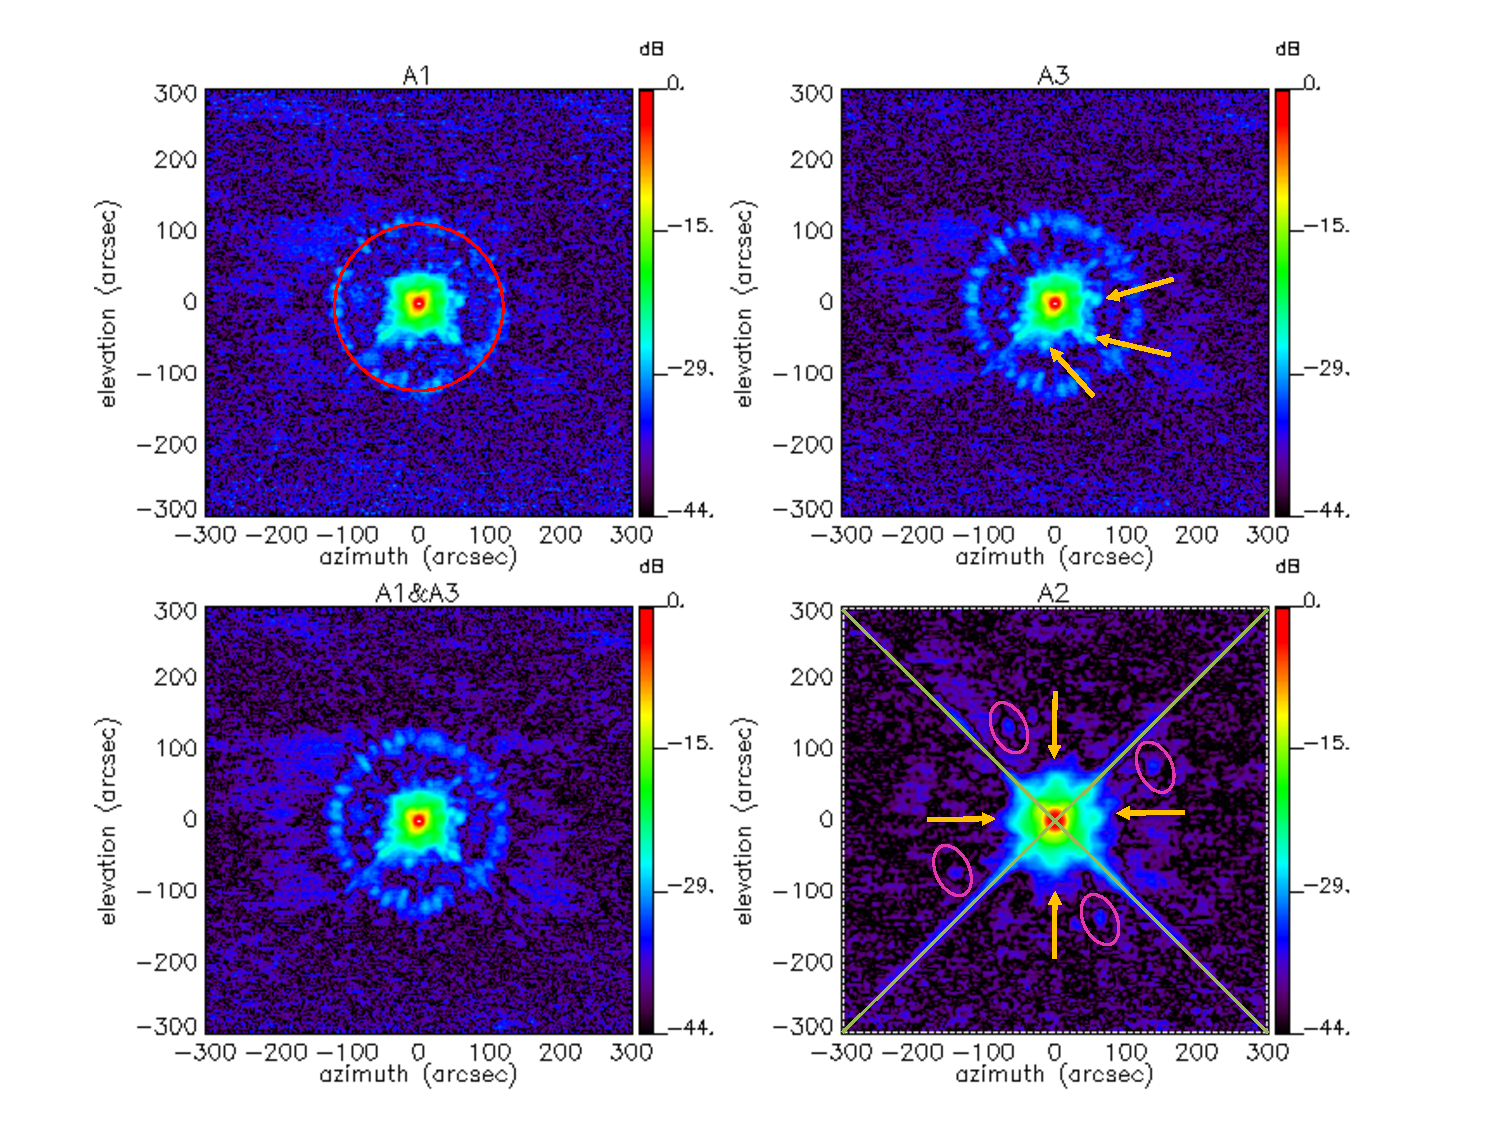
\includegraphics[width=0.9\linewidth]{Beams_features.pdf}
     
      \caption{Observed beam pattern. From upper left to lower right,
        beam maps of array 1 (labeled 'A1'), array 3 ('A3'), the
        combination of the 1.15mm arrays ('A1$\&$3') and the 2mm array
        ('A2') are shown in decibel. These maps, which consist of
        normalized combination of four long OTF scans of bright point
        sources, are in celestial coordinates and cover a sky area
        which extend over 10 arcmin. Colored lines evidence noticeable
        features of the NIKA2 Beam. Red circle: diffraction ring seen
        in 1-mm maps (the spokes are presumably caused by radial and
        azimuthal panel buckling (cf. Fig.4 in Greve et al. 2010));
        Perpendicular green lines: diffraction pattern caused by
        quadrupod secondary support structure (prominently seen in 2mm
        maps); Yellow arrows in the upper right pannel: pattern of 3
        spikes seen in 1mm maps of unknown origin; Yellow arrows in
        the lower right pannel: four symmetrical spokes of the first
        errorbeam; Pink ellipses: 4 spikes seen in 2mm maps.
      }
         \label{fig:beampattern}
\end{figure}


\subsection{On-sky calibration}
\label{On-sky calibration}
[JFL]
The planets Uranus and Neptune  were used as the primary calibrators to set the Jansky scale of the instrument.
Their flux densities at our conventional frequencies of 260~GHz and 150~GHz were adopted from the model in Moreno et al (...)
and updated at the mid-date of each of the two sessions in using planet geocentric distance
and viewing angle due to planetary oblateness provided by the JPL's HORIZONS Ephemeris.
About ten observations of these two planets with integration time of $\sim 20$ minutes were carried out at each session  
and resulted in high SNR maps with the main beam and side lobes apparent (e.g. Fig. \ref{fig:beampattern}).
Their total flux density were measured
from the maps both by gaussian fitting and aperture photometry within a radius of  $150''$ where cumulative flux density leveled off smoothly.
Both types of photometry provided consistent results with differences at the level of less than a few \% for all observations.
Line of sight opacities at 1 mm and 2mm derived from the data themselves as described
in $\S\ref{Atmospheric attenuation correction}$ were used to correct for atmospheric attenuation.
These final photometric measurements were compared to the reference
flux densities in plotting their ratios in Fig. \ref{fig:calibaccuracy}.

Over all, the flux density scale is stable at better than $7\%$ for all scans emcompassing
two one week long periods separated by two months, and despite the fact that the instrument was warmed up between the two sessions. 
As shown in Fig. \ref{fig:calibaccuracy}, the mean ratios for the three arrays is close to unity as expected since
the planets were used to set the Jansky scale in average over all the observations early in the processing. It could be
exactly unity in an iterative process [A DISCUTER]. It is noticeable
%that atmospheric conditions were significantly better during the  first session than the second. We find
that scatters around unity in Fig. \ref{fig:calibaccuracy}
are about twice smaller in the first session in significantly better weather than in the second session ; precisely, relative stabilities
are 3.6\%, 2.5\% and 2.9\% for arrays 1, 2, 3, respectively, for the first session with opacity $\tau_{1mm}$ between 0.05 and 0.3,
and correspondingly  5.3\%, 6.7\% and 8.6\% for the second with  $\tau_{1mm}$ between 0.25 and 0.6.
Hence, the main limitation in stability appears to be caused by residual atmospheric fluctuations in the processing. 

Nonetheless, this stability is satisfactory and similar to the level achieved by other modern instruments, e.g. SCUBA2 (Dempsey et al 2012).
The other limitation of the scale is absolute calibration that depends on the
accuracy of the Moreno et al's model which is estimated to be 5\% in the millimeter wavelength range. Hence, in combining both limitations,
the total uncertainty of calibration with NIKA2 is $10\%$ in mediocre atmospheric conditions and better than $10\%$ in fair condition. 

[JFL, en fabrication ] The absolute calibration has been checked with observations of the three secondary calibrators MWC349, NGC7027 and CRL2688.
Their flux densities are known from the literature (references + PdB monitoring for MWC349) and are stable at the .... level.
Color corrections have been done. Aperture photometry vs gaussian fitting. Results.


\begin{figure}[h]
   \centering
    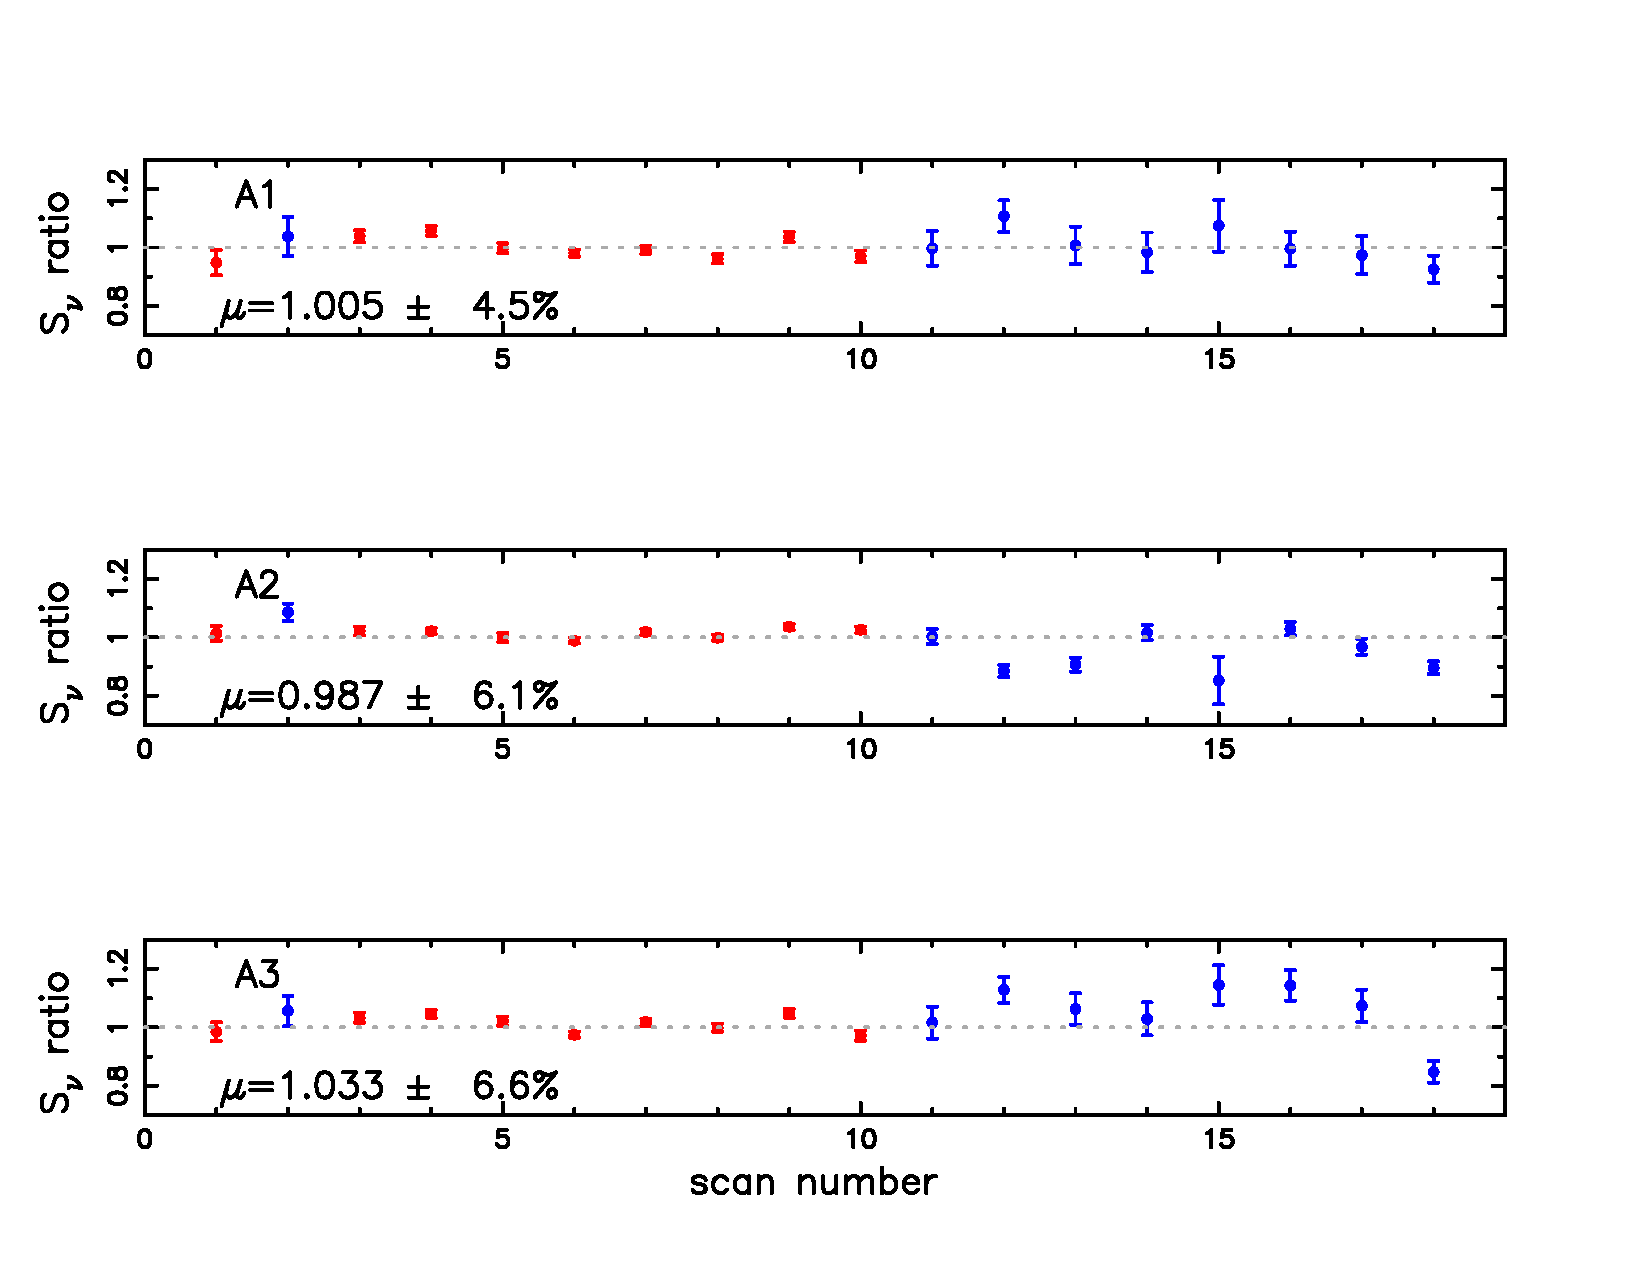
\includegraphics[angle=0,width=1.0\linewidth]{Ura_Nept_r9_10.pdf}     
    \caption{Comparison of  measured and reference flux densities of the primary calibrators Uranus (red) and Neptune (blue).
       Their ratios are shown for the three arrays A1 (1mm), A2 (2mm), A3(1mm).
      The mean ratio $\mu$ and relative scatter are provided for each array. The reference flux densities are from the Moreno et al ( ). 
      Scan numbers are time ordered : 1 to 10 is during the period 23-28 february 2017 and 11 to 18
      is during the  19-25 april 2017 period. Neptune was hardly visible at the telescope during the first session,
      and Uranus was not visible during the session.}
         \label{fig:calibaccuracy}
\end{figure}

\subsection{Noise and sensitivity}
\label{Noise and sensitivity}
We have investigated the noise properties and sensitivity of NIKA2 in various atmospheric conditions and for various types of sources including faint and bright ones.
We find that the evolution of the noise is consistent with background noise limited detectors both at 150 and 260 GHz. Furthermore, we find that when averaging
across scans the noise evolves consistently with the square root of the time of observation.
The averaged observed sensitivity assuming 2 mm of water vapor 
and at elevation of 60 degrees are 6 and 20 mJy.s$^{1/2}$ at 150 and 260 GHz, respectively. This corresponds to average mapping speed of 180 and 2000 arcmin$^2$/hr/mJy$^2$.

\subsection{Summary of performances}
We present in Table~\ref{sumperf} a summary of the main characteristic and performance of the NIKA2 instrument for one of the commissioning campaigns. From this table we conclude that NIKA2 behaves better than the initial specifications \cite{ltd16:2016} and approaches goal performance some cases.


\begin{table*}
\caption{Summary of the main instrumental characteristic and performance of the NIKA2 instrument. \label{sumperf}}
\begin{tabular}{|c|c|c|c|}
\hline
                          & Array 1 & Array3  & Array 2 \\
\hline
\hline

Central Frequency [GHz]   &         &         &         \\
Bandwidth         [GHz]   &   &     &       \\
Beam efficiency   [\% ]   & 55  49    & 53        &     75  70\\
Nummber of detectors      &         &         &         \\
                          &         &         &         \\ 
FWHM [arcsec]             &   11.2 11.18 0.24     &  11.2 11.08 0.34     &   17.7 17.33  0.07      
\\ 
Calibration errors []    &&& \\
Pointing errors    [arcsec]    & $<3$ && \\
\hline
\end{tabular}
\end{table*}

\section{Compact and extended sources mapping capabilities}
During commissioning and the science verification phase we have observed several compact and extended sources 
in order to check the NIKA2 mapping capabilities. Here we just concentrate in few sources to illustrate the main advantages of NIKA2 with respect to previous experiments.

\subsection{Point and compact sources} 
In Figure \ref{fig_compact_sources} we present maps of MWC349 (top) and the planet Pluto(bottom) at 150 (left) and 260 (righ) GHz.
The contours represent the SNR, which  blablabla .
We observe MWC349 and Pluto at the center of the maps and an extra source in the edge of the map. We find for MWC349 a flux of XXX Jy.

\begin{figure*}[h]
   \centering
   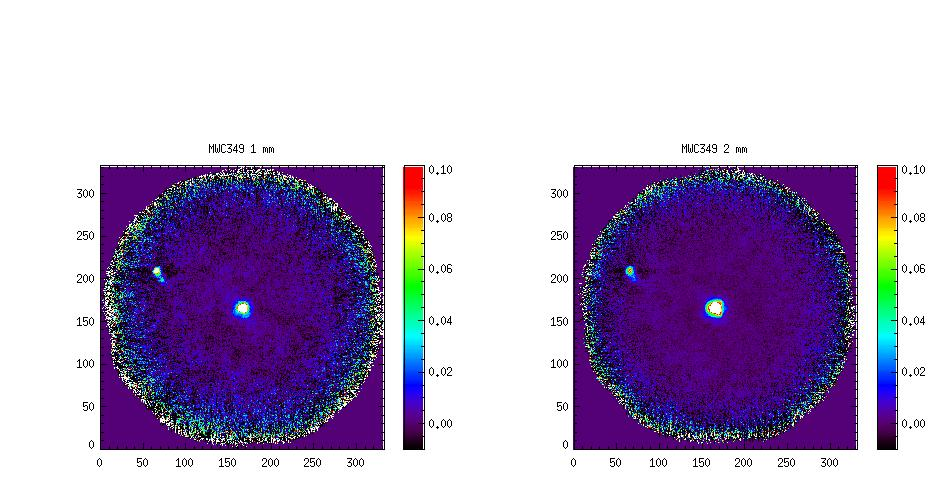
\includegraphics[width=.95\linewidth]{MWC349_v0.jpeg}
        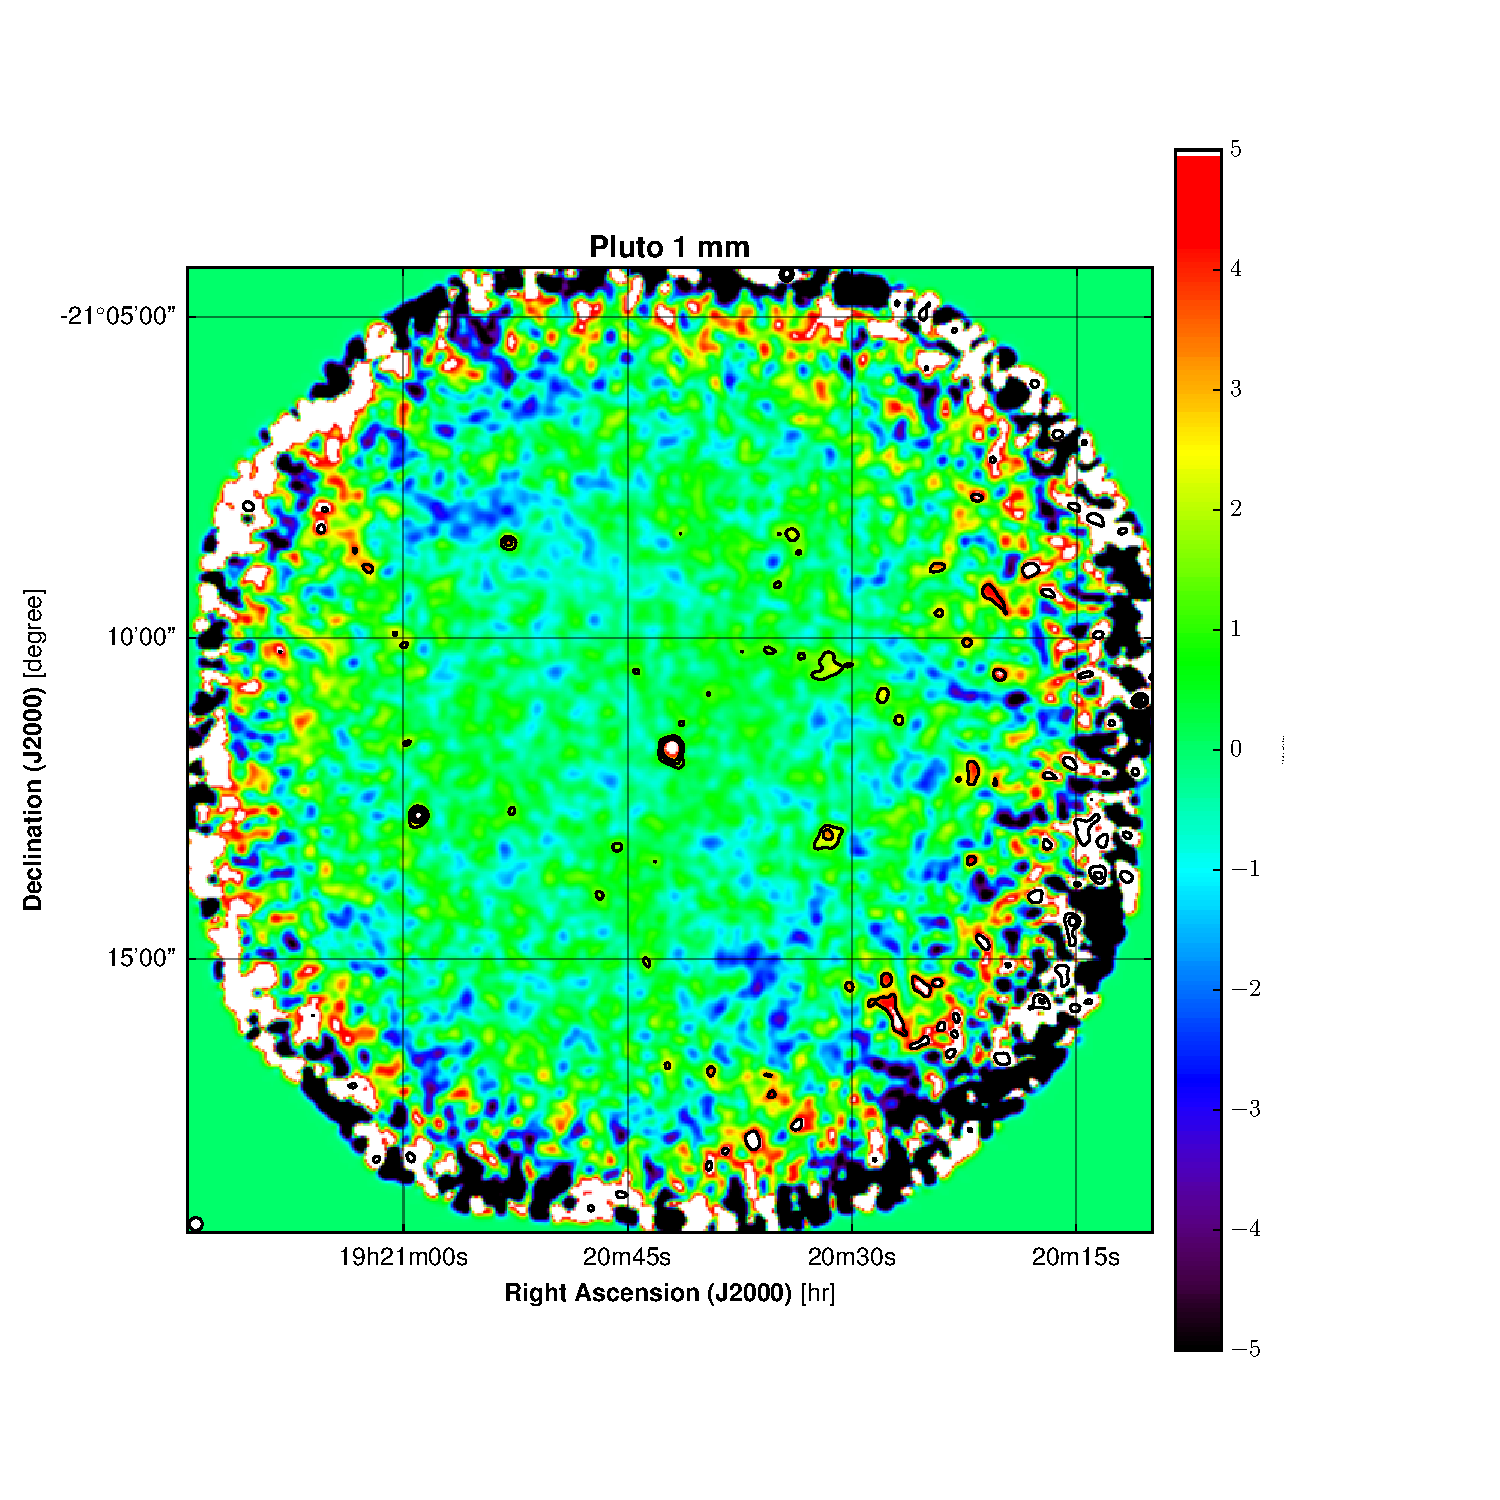
\includegraphics[width=.45\linewidth]{Pluto_1mm_map_snrcont.pdf}
    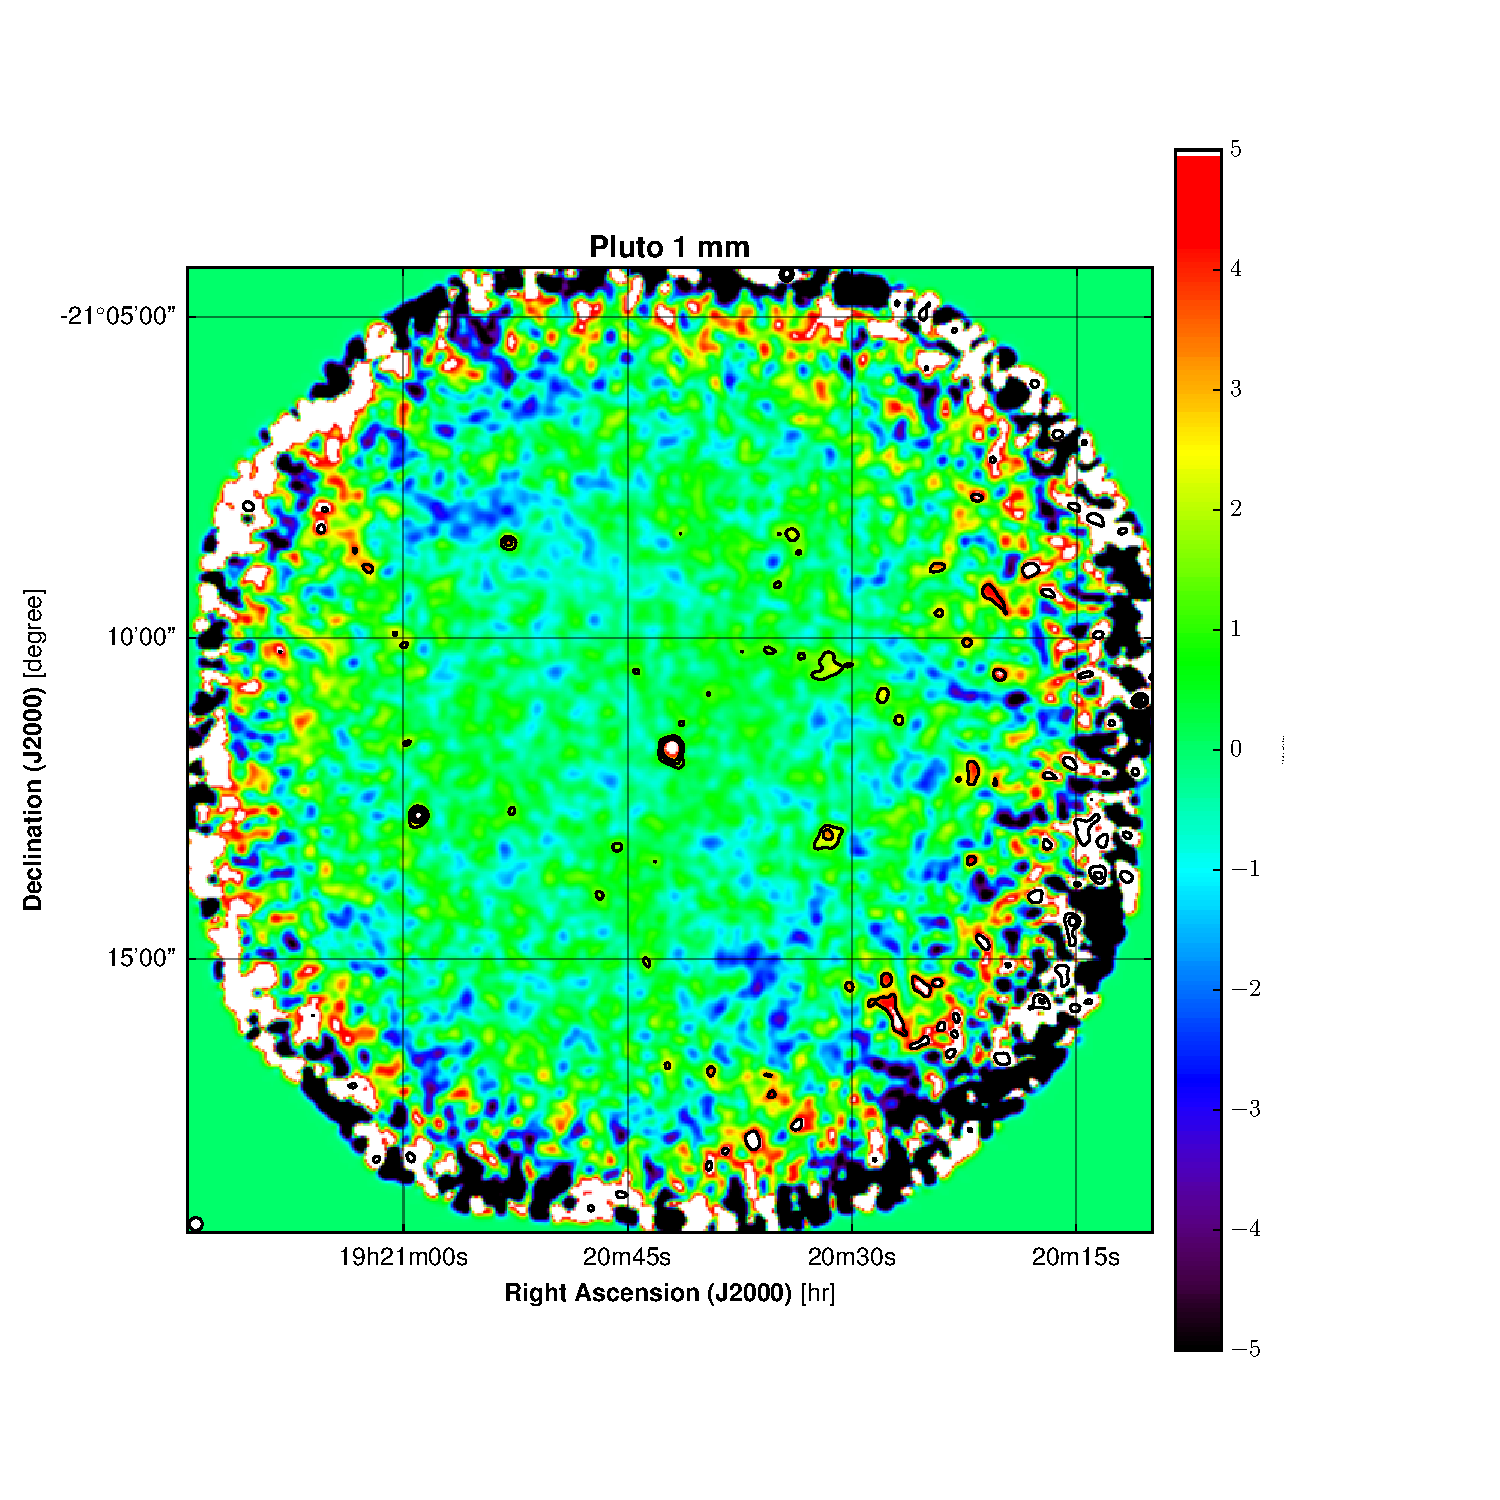
\includegraphics[width=.45\linewidth]{Pluto_1mm_map_snrcont.pdf}
      \caption{Top: Maps at 150 (left) and 260 (right) GHz of MWC349. Bottom: Maps at 150 (left) and 260 (right) GHz of the planet Pluto. {\bf change for better images}. 
         \label{fig_compact_sources}}
\end{figure*}


\subsection{Extended sources}
{\bf WE NEED TO FIND A SOURCE: why not this one (Fig.~\ref{fig:k3-50a}) (with improved display obviously
?}


\begin{figure*}[h]
   \centering
   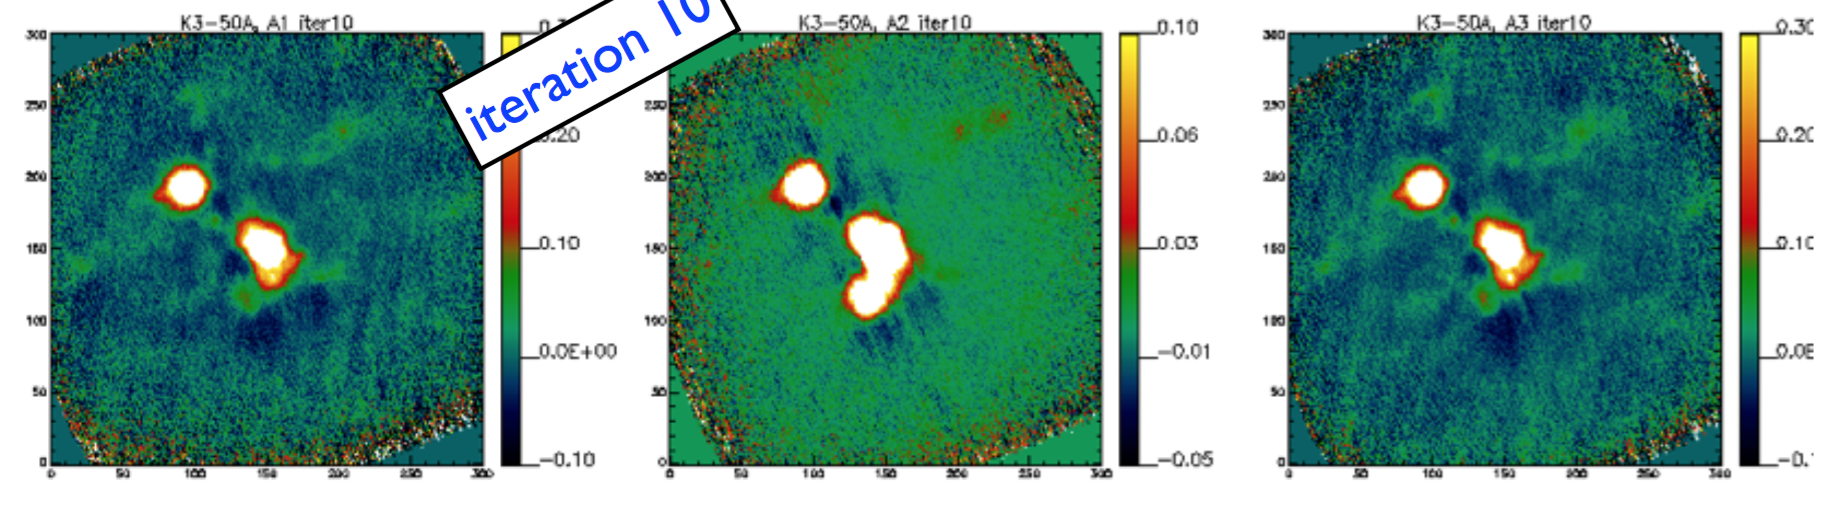
\includegraphics[width=.95\linewidth]{K3-50A.png}
   \caption{K3-50A place holder}. 
   \label{fig:k3-50a}
\end{figure*}




%WHO IN CHARGE ?? Contributions from many. Number of pages and figures you need. 1-2 possible ? 

%\subsection{Preliminary polarised maps}
%ALESSIA 

\section{Conclusions and future plans}

The NIKA2 instrument is permanently installed at the 30-meters telescope at Pico Veleta. In the present paper we have provided a general overwiew of the instrument, and given the first results obtained during the first three technical observing runs. The performance of the instrument are sufficiently good to satisfy the initial specifications already. Building on this base, NIKA2 is now allowed to enter the scientific commissioning phase. The goal is to open the instrument to the larger community during the Winter 2016/17. A more specific paper quoting final performance will be then be issued. 


\begin{acknowledgements}
{\it this is the current official NIKA2 Acknowledgements. please contact F.
Mayet if you would like to add smth.}.\\
We would like to thank the IRAM staff for their support during the campaigns. 
The NIKA dilution cryostat has been designed and built at the Institut N\'eel. 
In particular, we acknowledge the crucial contribution of the Cryogenics Group, and 
in particular Gregory Garde, Henri Rodenas, Jean Paul Leggeri, Philippe Camus. 
This work has been partially funded by the Foundation Nanoscience Grenoble, the LabEx FOCUS ANR-11-LABX-0013 and 
the ANR under the contracts "MKIDS", "NIKA" and ANR-15-CE31-0017. 
This work has benefited from the support of the European Research Council Advanced Grant ORISTARS 
under the European Union's Seventh Framework Programme (Grant Agreement no. 291294).
We acknowledge fundings from the ENIGMASS French LabEx (R. A. and F. R.), 
the CNES post-doctoral fellowship program (R. A.),  the CNES doctoral fellowship program (A. R.) and 
the FOCUS French LabEx doctoral fellowship program (A. R.).


\end{acknowledgements}

\begin{thebibliography}{16}
\expandafter\ifx\csname natexlab\endcsname\relax\def\natexlab#1{#1}\fi

\bibitem[{LTD16 2016}]{ltd16:2016}
Low Temperature Detectors LTD-16 Proceedings 2016,  Journal of Low
  Temperature Physics 184, numbers 1/2 and 3/4

\bibitem[{Monfardini {et~al.} 2011}]{Monfardini2011}
Monfardini, A., Benoit, A., Bideaud, A., {et~al.} 2011, 
The Astrophysical Journal Supplement 194, Issue 2, id. 24

\bibitem[{Catalano {et~al.} 2014}]{Catalano2014}
Catalano, A., Calvo, M., Ponthieu, N., {et~al.} 2014, 
Astronomy \& Astrophysics 569, id.A9

\bibitem[{Adam {et~al.} 2014}]{Adam2014}
Adam, R., Comis, B., Mac\'ias-P\'erez, J.-F., {et~al.} 2014, 
Astronomy \& Astrophysics 569, id.A66

\bibitem[{Day {et~al.} 2003}]{Day2003}
Day, P.~K., LeDuc, H.~G., Mazin, B.~A., Vayonakis, A., \& Zmuidzinas, J. 2003,
  Nature, 425, 817

\bibitem[{Doyle {et~al.} 2010}]{Doyle2010}
Doyle, S., Mauskopf, P., Zhang, J., {et~al.} 2008{\natexlab{a}}, in Millimeter
  and Submillimeter Detectors and Instrumentation for Astronomy IV, Proc. SPIE,
  7020, 702009

\bibitem[{Calvo {et~al.} 2010}]{Calvo2010}
Calvo, M., Giordano, C., Battiston, R., {et~al.} 2010, 
Experimental Astronomy 28, Issue 2-3, 185

\bibitem[{Roesch {et~al.} 2012}]{Roesch2012}
Roesch, M., Benoit, A., Bideaud, A., {et~al.} 2012, 
ISSTT2011 Workshop, arXiv:1212.4585

\bibitem[{Goupy {et~al.} 2016}]{Goupy2016}
Goupy, J., Adane, A., Benoit, A., {et~al.} 2016, 
Journal of Low Temperature Physics xxx, xxx, xxx

\bibitem[{Pisano {et~al.} 2016}]{Pisano2016}
Pisano, G., Xxx, X., Bbb, X., {et~al.} 2016, 
In preparation

\bibitem[{Bourrion {et~al.} 2012}]{Bourrion2012}
Bourrion, O., Vescovi, C., Bouly, J.L., {et~al.} 2012, 
Journal of Instrumentation, vol 7, P07014, arXiv:1204.1415

\bibitem[{Bourrion {et~al.} 2016}]{Bourrion2016}
Bourrion, O., Benoit, A., Bouly, J.L., {et~al.} 2016, 
Journal of Instrumentation, vol. 11, P11001, arXiv:1602.01288

\bibitem[{Swenson {et~al.} 2010}]{Swenson2010}
Swenson, L. J., Cruciani, A., Benoit, A., {et~al.} 2010, 
Applied Physics Letters 96, Issue 26, id. 263511

\bibitem[{Durand 2008}]{Durand2008}
Durand, T., 2008, 
PhD Thesis, Universit\' e de Grenoble

\bibitem[{Calvo {et~al.} 2013}]{Calvo2013}
Calvo, M., Roesch, M., D\'esert, F.-X., {et~al.} 2013, 
Astronomy \& Astrophysics 551, id.L12

\bibitem[{Pardo {et~al.} 2002}]{2001IEEE....49.1683C}
Pardo J.~R., Cernicharo J., Serabyn E., 2002, 
IEEE, 49, 1683 - 1694


\end{thebibliography}

%\bibliographystyle{aa}
%\bibliography{biblio_NIKA2} 

\end{document}



%%%%%%%%%%%%%%%%%%%%%%%%%%%%%%%%%%%%%%%%%%%%%%%%%%%%%%%%%%%%%%
Examples for figures using graphicx
A guide "Using Imported Graphics in LaTeX2e"  (Keith Reckdahl)
is available on a lot of LaTeX public servers or ctan mirrors.
The file is : epslatex.pdf
%%%%%%%%%%%%%%%%%%%%%%%%%%%%%%%%%%%%%%%%%%%%%%%%%%%%%%%%%%%%%%

%_____________________________________________________________
%                 A figure as large as the width of the column
%-------------------------------------------------------------
   \begin{figure}
   \centering
   \includegraphics[width=\textwidth]{empty.eps}
      \caption{Vibrational stability equation of state
               $S_{\mathrm{vib}}(\lg e, \lg \rho)$.
               $>0$ means vibrational stability.
              }
         \label{FigVibStab}
   \end{figure}
%
%_____________________________________________________________
%                                    One column rotated figure
%-------------------------------------------------------------
   \begin{figure}
   \centering
   \includegraphics[angle=-90,width=3cm]{empty.eps}
      \caption{Vibrational stability equation of state
               $S_{\mathrm{vib}}(\lg e, \lg \rho)$.
               $>0$ means vibrational stability.
              }
         \label{FigVibStab}
   \end{figure}
%
%_____________________________________________________________
%                        Figure with caption on the right side
%-------------------------------------------------------------
   \begin{figure}
   \centering
   \includegraphics[width=3cm]{empty.eps}
      \caption{Vibrational stability equation of state
               $S_{\mathrm{vib}}(\lg e, \lg \rho)$.
               $>0$ means vibrational stability.
              }
         \label{FigVibStab}
   \end{figure}
%
%_____________________________________________________________
%
%_____________________________________________________________
%                                Figure with a new BoundingBox
%-------------------------------------------------------------
   \begin{figure}
   \centering
   \includegraphics[bb=10 20 100 300,width=3cm,clip]{empty.eps}
      \caption{Vibrational stability equation of state
               $S_{\mathrm{vib}}(\lg e, \lg \rho)$.
               $>0$ means vibrational stability.
              }
         \label{FigVibStab}
   \end{figure}
%
%_____________________________________________________________
%
%_____________________________________________________________
%                                      The "resizebox" command
%-------------------------------------------------------------
   \begin{figure}
   \resizebox{\textwidth}{!}
            {\includegraphics[bb=10 20 100 300,clip]{empty.eps}
      \caption{Vibrational stability equation of state
               $S_{\mathrm{vib}}(\lg e, \lg \rho)$.
               $>0$ means vibrational stability.
              }
         \label{FigVibStab}
   \end{figure}
%
%______________________________________________________________
%
%_____________________________________________________________
%                                             Simple A&A Table
%_____________________________________________________________
%
\begin{table}
\caption{Nonlinear Model Results}             % title of Table
\label{table:1}      % is used to refer this table in the text
\centering                          % used for centering table
\begin{tabular}{c c c c}        % centered columns (4 columns)
\hline\hline                 % inserts double horizontal lines
HJD & $E$ & Method\#2 & Method\#3 \\    % table heading
\hline                        % inserts single horizontal line
   1 & 50 & $-837$ & 970 \\      % inserting body of the table
   2 & 47 & 877    & 230 \\
   3 & 31 & 25     & 415 \\
   4 & 35 & 144    & 2356 \\
   5 & 45 & 300    & 556 \\
\hline                                   %inserts single line
\end{tabular}
\end{table}
%
%_____________________________________________________________
%                                             Two column Table
%_____________________________________________________________
%
\begin{table*}
\caption{Nonlinear Model Results}
\label{table:1}
\centering
\begin{tabular}{c c c c l l l }     % 7 columns
\hline\hline
                      % To combine 4 columns into a single one
HJD & $E$ & Method\#2 & \multicolumn{4}{c}{Method\#3}\\
\hline
   1 & 50 & $-837$ & 970 & 65 & 67 & 78\\
   2 & 47 & 877    & 230 & 567& 55 & 78\\
   3 & 31 & 25     & 415 & 567& 55 & 78\\
   4 & 35 & 144    & 2356& 567& 55 & 78 \\
   5 & 45 & 300    & 556 & 567& 55 & 78\\
\hline
\end{tabular}
\end{table*}
%
%_____________________________________________________________
%                                          Table with foonotes
%-------------------------------------------------------------
%
\begin{table}
\begin{minipage}[t]{\columnwidth}
\caption{LHNW source catalogue.}
\label{catalog}
\centering
\renewcommand{\footnoterule}{}  % to avoid a line before footnotes
\begin{tabular}{lccccc}
\hline \hline
ID& RA     &  Dec    & {\it S/N} & Flux  \\
~ &(J2000) & (J2000) &~    & [{\rm mJy}] \\
\hline
   LHJ10  &10:32:02.4  &     +58:80:09  &   8  &    97 $\pm$  15\\
   LHJ10  &10:33:08.8  &     +58:80:30  &   5  &    80 $\pm$  16\\
   LHJ10  &10:34:45.1  &     +57:47:33\footnote{Text of the footnote}
                                               &   5  &    48 $\pm$  10\\
   LHJ10  &10:32:49.7  &     +57:37:19  &   5  &    56 $\pm$  11\\
   LHJ10  &10:33:52.1  &     +58:40:30\footnote{Text of the footnote}
                                               &   4  &    55 $\pm$  14\\
   LHJ10  &10:33:04.3  &     +57:36:37  &   4  &    55 $\pm$  14\\
   LHJ10  &10:35:50.4  &     +57:30:05  &   4  &    49 $\pm$  11\\
\hline
\end{tabular}
\end{minipage}
\end{table}
%
%_____________________________________________________________
%                                 A rotated Table in landscape
%  In the preamble, use:   \usepackage{lscape}
%-------------------------------------------------------------
\begin{landscape}
\begin{table*}
\caption{Summary for ISOCAM sources with mid-IR excess
(YSO candidates).}\label{YSOtable}
\centering
\begin{tabular}{crrlcl}
\hline\hline
ISO-L1551 & $F_{6.7}$~[mJy] & $\alpha_{6.7-14.3}$
& YSO type$^{d}$ & Status & Comments\\
\hline
  \multicolumn{6}{c}{\it New YSO candidates}\\ % To combine 6 columns into a single one
\hline
  1 & 1.56 $\pm$ 0.47 & --    & Class II$^{c}$ & New & Mid\\
  2 & 0.79:           & 0.97: & Class II ?     & New & \\
  3 & 4.95 $\pm$ 0.68 & 3.18  & Class II / III & New & \\
  5 & 1.44 $\pm$ 0.33 & 1.88  & Class II       & New & \\
\hline
  \multicolumn{6}{c}{\it Previously known YSOs} \\
\hline
  61 & 0.89 $\pm$ 0.58 & 1.77 & Class I & \object{HH 30} & Circumstellar disk\\
  96 & 38.34 $\pm$ 0.71 & 37.5& Class II& MHO 5          & Spectral type\\
\hline
\end{tabular}
\end{table*}
\end{landscape}
%
%_____________________________________________________________
%                              Table longer than a single page
%  In the preamble, use:              \usepackage{longtable}
%-------------------------------------------------------------
%          All long tables have to be placed at the end, after
%                                        \end{thebibliography}
%
% In the text, at the place where the large table should appear
% add the command:
\addtocounter{table}{1}
% Tables counters will be well numbered.
%
\end{thebibliography}
% If table 2
\longtab{2}{
\begin{longtable}{lllrrr}
\caption{\label{kstars} Sample stars with absolute magnitude}\\
\hline\hline
Catalogue& $M_{V}$ & Spectral & Distance & Mode & Count Rate \\
\hline
\endfirsthead
\caption{continued.}\\
\hline\hline
Catalogue& $M_{V}$ & Spectral & Distance & Mode & Count Rate \\
\hline
\endhead
\hline
\endfoot
%%
Gl 33    & 6.37 & K2 V & 7.46 & S & 0.043170\\
Gl 66AB  & 6.26 & K2 V & 8.15 & S & 0.260478\\
Gl 68    & 5.87 & K1 V & 7.47 & P & 0.026610\\
         &      &      &      & H & 0.008686\\
Gl 86
\footnote{Source not included in the HRI catalog. See Sect.~5.4.2 for details.}
         & 5.92 & K0 V & 10.91& S & 0.058230\\
\end{longtable}
}% End \longtab
%
%_____________________________________________________________
%                              Table longer than a single page
%                                             and in landscape
%  In the preamble, use:       \usepackage{longtable,lscape}
%-------------------------------------------------------------
%          All long tables have to be placed at the end, after
%                                        \end{thebibliography}
%
% In the text, at the place where the large table should appear
% add the command:
\addtocounter{table}{1}
% Tables counters will be well numbered.
%
\end{thebibliography}
% If table 2
\longtabL{2}{
\begin{landscape}
\begin{longtable}{lllrrr}
\caption{\label{kstars} Sample stars with absolute magnitude}\\
\hline\hline
Catalogue& $M_{V}$ & Spectral & Distance & Mode & Count Rate \\
\hline
\endfirsthead
\caption{continued.}\\
\hline\hline
Catalogue& $M_{V}$ & Spectral & Distance & Mode & Count Rate \\
\hline
\endhead
\hline
\endfoot
%%
Gl 33    & 6.37 & K2 V & 7.46 & S & 0.043170\\
Gl 66AB  & 6.26 & K2 V & 8.15 & S & 0.260478\\
Gl 68    & 5.87 & K1 V & 7.47 & P & 0.026610\\
         &      &      &      & H & 0.008686\\
Gl 86
\footnote{Source not included in the HRI catalog. See Sect.~5.4.2 for details.}
         & 5.92 & K0 V & 10.91& S & 0.058230\\
\end{longtable}
\end{landscape}
}% End \longtabL
%
% Online Material
%_____________________________________________________________
%        Online appendices have to be placed at the end, after
%                                        \end{thebibliography}
%-------------------------------------------------------------
\end{thebibliography}

\Online

\begin{appendix} %First online appendix
\section{Background galaxy number counts and shear noise-levels}
Because the optical images used in this analysis...

\begin{figure*}
\centering
\includegraphics[width=16.4cm,clip]{1787f24.ps}
\caption{Plotted above...}
\label{appfig}
\end{figure*}

Because the optical images...
\end{appendix}

\begin{appendix} %Second online appendix
These studies, however, have faced...
\end{appendix}

\end{document}
%
%_____________________________________________________________
%        Some tables or figures are in the printed version and
%                      some are only in the electronic version
%-------------------------------------------------------------
%
% Leave all the tables or figures in the text, at their right place
% and use the commands \onlfig{}{} and \onltab{}{}. These elements
% will be automatically placed at the end, in the section
% Online material.

\documentclass{aa}
...
\begin{document}
text of the paper...
\begin{figure*}%f1
\includegraphics[width=10.9cm]{1787f01.eps}
\caption{Shown in greyscale is a...}
\label{cl12301}}
\end{figure*}
...
from the intrinsic ellipticity distribution.
% Figure 2 available electronically only
\onlfig{2}{
\begin{figure*}%f2
\includegraphics[width=11.6cm]{1787f02.eps}
\caption {Shown in greyscale...}
\label{cl1018}
\end{figure*}
}

% Figure 3 available electronically only
\onlfig{3}{
\begin{figure*}%f3
\includegraphics[width=11.2cm]{1787f03.eps}
\caption{Shown in panels...}
\label{cl1059}
\end{figure*}
}

\begin{figure*}%f4
\includegraphics[width=10.9cm]{1787f04.eps}
\caption{Shown in greyscale is...}
\label{cl1232}}
\end{figure*}

\begin{table}%t1
\caption{Complexes characterisation.}\label{starbursts}
\centering
\begin{tabular}{lccc}
\hline \hline
Complex & $F_{60}$ & 8.6 &  No. of  \\
...
\hline
\end{tabular}
\end{table}
The second method produces...

% Figure 5 available electronically only
\onlfig{5}{
\begin{figure*}%f5
\includegraphics[width=11.2cm]{1787f05.eps}
\caption{Shown in panels...}
\label{cl1238}}
\end{figure*}
}

As can be seen, in general the deeper...
% Table 2 available electronically only
\onltab{2}{
\begin{table*}%t2
\caption{List of the LMC stellar complexes...}\label{Properties}
\centering
\begin{tabular}{lccccccccc}
\hline  \hline
Stellar & RA & Dec & ...
...
\hline
\end{tabular}
\end{table*}
}

% Table 3 available electronically only
\onltab{3}{
\begin{table*}%t3
\caption{List of the derived...}\label{IrasFluxes}
\centering
\begin{tabular}{lcccccccccc}
\hline \hline
Stellar & $f12$ & $L12$ &...
...
\hline
\end{tabular}
\end{table*}
}
%
%-------------------------------------------------------------
%     For the online material, table longer than a single page
%                 In the preamble, use: \usepackage{longtable}
%       or for landscape option: \usepackage{longtable,lscape}
%-------------------------------------------------------------
\documentclass{aa}
\usepackage[varg]{txfonts}
\usepackage{graphicx}
\usepackage{longtable}

\begin{document}
text of the paper
% Table will be print automatically at the end, in the section Online material.
\onllongtab{3}{
\begin{longtable}{lrcrrrrrrrrl}
\caption{Line data and abundances ...}\\
\hline
\hline
Def & mol & Ion & $\lambda$ & $\chi$ & $\log gf$ & N & e &  rad & $\delta$ & $\delta$
red & References \\
\hline
\endfirsthead
\caption{Continued.} \\
\hline
Def & mol & Ion & $\lambda$ & $\chi$ & $\log gf$ & B & C &  rad & $\delta$ & $\delta$
red & References \\
\hline
\endhead
\hline
\endfoot
\hline
\endlastfoot
A & CH & 1 &3638 & 0.002 & $-$2.551 &  &  &  & $-$150 & 150 &  Jorgensen et al. (1996) \\
\end{longtable}
}% End onllongtab

% Or for landscape, large table:

\onllongtabL{3}{
\begin{landscape}
\begin{longtable}{lrcrrrrrrrrl}
...
\end{longtable}
\end{landscape}
}% End onllongtabL
